\documentclass[a4paper, 10pt, ]{article}
\usepackage{polski}
\usepackage[utf8]{inputenc}
\usepackage{graphicx}
\graphicspath{ {./images/} }
\usepackage[polish]{babel}
\usepackage{enumerate}
\usepackage{paralist}
\usepackage[margin=1in]{geometry}
\usepackage{yhmath}
\usepackage{latexsym}
\usepackage{amsmath,esint}
 \usepackage{ulem}
 \usepackage{color}


\title{Ultrapack, czyli POFA od zera do bohatera}
\author{Wersja 2.0}
\date{30 czerwca 2014}

\newenvironment{task}{\setlength{\parindent}{0cm}\noindent}{}
\newenvironment{solution}{\noindent \textbf{ Rozwiązanie:\newline} \setlength{\parindent}{0cm}\noindent}{}

%% \renewcommand\thesection{Zadanie \arabic{section}.}
\graphicspath{{images/}}
\begin{document}
\maketitle
\begin{center}
	
\includegraphics{images/logo}
\end{center}

\thispagestyle{empty}
\newpage
\section*{ }

\newpage
\section*{Errata}
Przepraszamy za błędy, które znajdziecie w opracowaniach. Zadania rozkminiane były dniami i nocami, pod presją czasu. Liczymy, że kolejne semestry ulepszą to tak, by w przyszłości nikt nie miał problemu z zaliczeniem:). Zadania teoretyczne są opisane zbyt szczegółowo, sądzę, że nie ma potrzeby na tak wielkie zaangażowanie i znajomość wzorów, wystarczy pokazać prowadzącym, że potrafisz myśleć i mniej więcej coś kojarzysz. \sout{Jeśli chodzi o 3 ośrodki to nasze obliczenia są zbędne. Dowiedzieliśmy sie dopiero po egzaminie :D. Są łatwiejsze sposoby na rozwiązanie.} Zbiór zadań powstał dzięki 17 egzaminom znalezionym w internecie:) nie ma zadania, które się nie powtórzyło(dwa, trzy, cztery a nawet piętnaście razy widzieliśmy to samo:) ). Powodzenia z pofką! Nie jest aż tak źle.
\begin{itemize}
\item Wiola Kruk
\item Paweł Borkowski
\item Janek Kalmus
\item Piotrek Synal
\item Wojtek Chaberek
\item Walczyk Mateusz
\end{itemize}
Update do wersji 1.3
\begin{itemize}
\item Staszek Aleksiński
\item Damgad
\item dr Salski
\end{itemize}
Z pomocą Marcin Bychawskiego i paru innych osób z forum. Dzięki!\\ Wszystkiego nie poprawiliśmy, więc przyszłe pokolenia mogą się jeszcze wykazać.\\

\section*{Przyszłe pokolenia się wykazują (update v2.0)}
\begin{itemize}
\item Zredagował: Marcin Skwarek, Rafał Trojak
\item Konsultacje merytoryczne: Bartłomiej Garnek
\item Konsultacje techniczne: Marek Baranowski
\end{itemize}

Pamiętajcie, że zadania nie są w żaden sposób uporządkowane względem trudności.\\
Jeśli jest ktoś, kto chciałby coś poprawić, dodać, dopisać to dysponujemy plikami, które chętnie udostępnimy zainteresowanym.
\newpage
\textcolor{red}{Dziwnie tak zaczynać od lewej. \#AdamLewak}
\section*{ }

\newpage


\section*{Zadanie 1.}

\begin{task}
Które z poniższych par wyrażeń nie opisują fali płaskiej w próżni i dlaczego? Które z par wyrażeń opisują taką falę i jakie wtedy muszą być spełnione warunki:
\begin{enumerate}[a)]
\item $ E(t, r) = {i}_{z}{E}_{0}sin(\omega t - {\beta}_{z}z), H(t, r) = {i}_{y}{H}_{0}sin(\omega t - {\beta}_{z}z) $
\item $ E(t, r) = {i}_{z}{E}_{0}sin(\omega t - {\beta}_{x}x), H(t, r) = {i}_{z}{H}_{0}sin(\omega t - {\beta}_{x}x) $
\item $ E(t, r) = {i}_{z}{E}_{0}sin(\omega t - {\beta}_{x}x), H(t, r) = {i}_{y}{H}_{0}sin(\omega t - {\beta}_{x}x) $
\item $ E(t, r) = {i}_{z}{E}_{0}sin(\omega t)cos({\beta}_{y}y), H(t, r) = {i}_{x}{H}_{0}cos(\omega t)sin({\beta}_{z}z) $
\item $ E(t, r) = {i}_{x}{E}_{0}sin(\omega t)sin({\beta}_{y}y), H(t, r) = {i}_{z}{H}_{0}cos(\omega t)cos({\beta}_{y}y) $\\
\end{enumerate}
\end{task}

\begin{solution}
\begin{enumerate}[a)]
\item Nie są spełnione warunki rozchodzenia się fali płaskiej.
\item Nie są spełnione warunki rozchodzenia się fali płaskiej
\item $ \vec{S} = \vec{E}\times\vec{H} = \left[ \begin{matrix} \vec{{i}_{x}} & \vec{{i}_{y}}  & \vec{{i}_{z}}  \\ 0 & 0 & 1 \\ 0 & 1 & 0 \end{matrix} \right] = -\vec{{i}_{x}} $, wektor Poyntinga nie zgadza się więc z kierunkiem rozchodzenia fali
\item Nie, wektor Poyntinga niezgodny z $\vec{k}$.
\item Nie, wektor Poyntinga niezgodny z $\vec{k}$.
\end{enumerate}
\end{solution}
\section*{Zadanie 2.}
\begin{task}
Wytłumaczyć jaki zachodzi związek między wirowością i potencjalnością pola. Odnosząc się do tego związku oraz do równań Maxwella, wyjaśnić kiedy można prawidłowo zdefiniować napięcie dla pól stałych i zmiennych w czasie? W jakich warunkach można poprawnie zdefiniować napięcie w linii TEM?\\
\end{task}

\begin{solution}

\textbf{Wirowość (rotacja)} - jeśli pole jest bezwirowe, posiada potencjał. Każde pole posiadające potencjał jest bezwirowe.
$$\oint\vec{E}dl=\iint\nabla\times\vec{E}d\vec{s}=0 \ \ \ \ \ \ \int\limits_{A}^{B}\vec{E}d\vec{l}=U$$
\textbf{Pola zmienne w czasie.} Zmiany indukcji magnetycznej powodują powstanie wirowego pola elektrycznego, zaś zmiany indukcji elektrycznej - magnetycznego.\\Pola elektryczne i magnetyczne nie dają się odseparować, dlatego używamy pojęcia pole elektromagnetyczne.\\W przypadku gdy pola są statyczne (rotacja pola E i rotacja pola H są zerowe wgzlędem czasu) żadne z równań Maxwella nie zawiera jednocześnie pól elektrycznego i magnetycznego, pola te są niezależne.

$$\nabla\times\vec{E}=\cfrac{\partial\vec{B}}{\partial t}\ \ \ \ \ \ \ \nabla\times\vec{H}=\vec{J}+\cfrac{\partial\vec{D}}{\partial t}\ \ \ \ \ \ \ \ \ U_{A,B}=\int\limits_{A}^{B}\vec{E}d\vec{l}$$

W przypadku linii TEM pole elektryczne jest bezwirowe w przekroju poprzecznym linii. Jeśli punkty A i B leżą w tej samej płaszczyźnie poprzecznej $z=const$ oraz jeżeli droga po której całkujemy leży w tej płaszczyźnie to rotacja pola E i napięcie między tymi punktami są definicjami poprawnymi i jednostronnymi.
\end{solution}
\section*{Zadanie 3.}
\begin{task}
Narysować obwiednię pól $E$, $H$, $B$, jaka powstanie w wyniku padania fali o częstotliwości $0.5\ GHz$ rozchodzącej się w kierunku $+Ox$ w układzie trzech ośrodków:\\
I $\hspace{1cm}$ $\epsilon=2\epsilon_{0} \hspace{1cm} \mu=\mu_{0} \hspace{1cm} \sigma=0 \hspace{4cm}$ dla $x<0$\\
II $\hspace{0.86cm}$ $\epsilon=2\epsilon_{0} \hspace{0.97cm} \mu=2\mu_{0} \hspace{0.85cm} \sigma=0 \hspace{4cm}$ dla $0\le x<a$\\
III $\hspace{0.73cm}$ $\epsilon=\epsilon_{0} \hspace{1.15cm} \mu=4\mu_{0} \hspace{0.84cm} \sigma=0 \hspace{4cm}$ dla $a\le x$\\
Przy a=15cm. W każdą obwiednię wpisać kilka krzywych obrazujących chwilowe rozkłady pola.\\
\textbf{Uwaga:} Zwrócić uwagę na możliwość zmiany długości fali przy przekraczaniu granicy ośrodków.\\
\end{task}

\begin{solution}

$$Z_{1}=Z_{0}\sqrt{\cfrac{\mu_{r}}{\epsilon_{r}}}=60\sqrt{2}\pi \ \ \ Z_{2}=Z_{0}\sqrt{\cfrac{2}{2}}=120\pi\ \ \ \ Z_{3}=Z_{0}\sqrt{\cfrac{4}{1}}=240\pi$$\\
$\beta_{2}=\cfrac{20}{3}\pi \ \ \implies \ \lambda_{2}=0.3m=2d \ \implies$ w 2. ośrodku mieści się dokładnie pół długości fali, więc: $Z_{in}=Z_{3}$
$$\Gamma_{1,2}=\cfrac{Z_{in}-Z_{1}}{Z_{in}+Z_{1}}\approx\cfrac{1}{2} \ \ \ \ \Gamma_{2,3}=\cfrac{Z_{3}-Z_{2}}{Z_{3}+Z_{2}}=\cfrac{1}{3}$$

$$WFS_{1}=\cfrac{1+|\Gamma_{1,2}|}{1-|\Gamma_{1,2}|}=3 \ \ \ \ WFS_{2}=\cfrac{1+|\Gamma_{2,3}|}{1-|\Gamma_{2,3}|}=2$$ 

$$E_{1max}=\Gamma_{1,2}E_{0}+E_{0}=\cfrac{3}{2}E_{0} \ \ \ \ E_{1min}=\cfrac{E_{1max}}{WFS_{1}}=\cfrac{1}{2} \ \ \ \ E_{2max}=E_{1max} \ \ \ E_{2min}=\cfrac{E_{2max}}{WFS_{2}}=\cfrac{3}{4}E_{0}$$

\begin{center}
$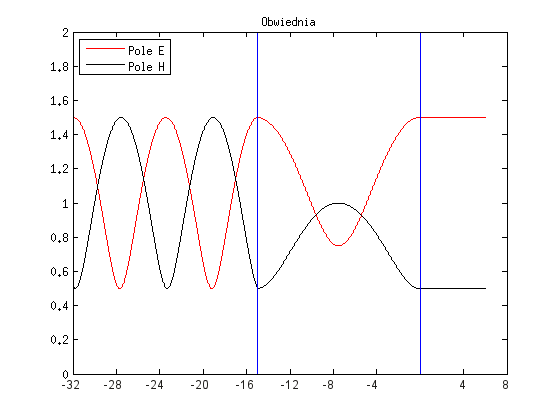
\includegraphics[scale=1]{../images/3_1}$\\
\end{center}
\begin{center}
$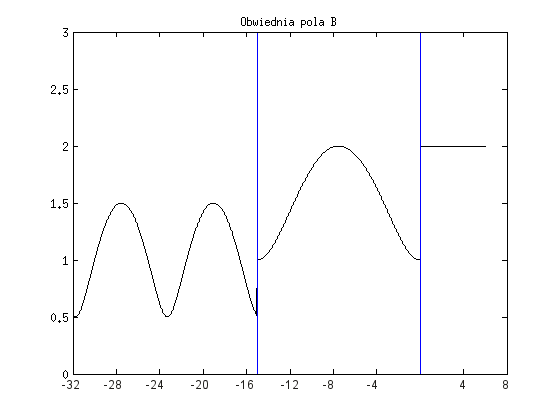
\includegraphics[scale=1]{images/3_2}$\\
\end{center}

\end{solution}
\section*{Zadanie 4.}
\begin{task}
Rozważamy rozkład pola rodzaju $H_{11}$ w falowodzie prostokątnym o szerokości $a$(w kierunku osi $Ox$), wysokości $h$(w kierunku osi $Oy$). Narysować rozkłady prądów powierzchniowych oraz zaznaczyć miejsca maksimów ładunków powierzchniowych na:
\begin{enumerate}[a)]
\item ściance dolnej (y=0) oraz bocznej (x=0) przy założeniu fali bieżącej rozchodzącej się w kierunku $+Oz$
\item ściance dolnej (y=0), bocznej(x=0) oraz ściance z idealnego przewodnika przegradzającej falowód w płaszczyźnie $x=0$, przy założeniu padania fali od strony ujemnych wartości współrzędnej $z$.\\
\end{enumerate}
\end{task}

\begin{solution}

\begin{enumerate}[a)]
	\item Rozkład pól dla fali bieżącej 
	\begin{center}
	$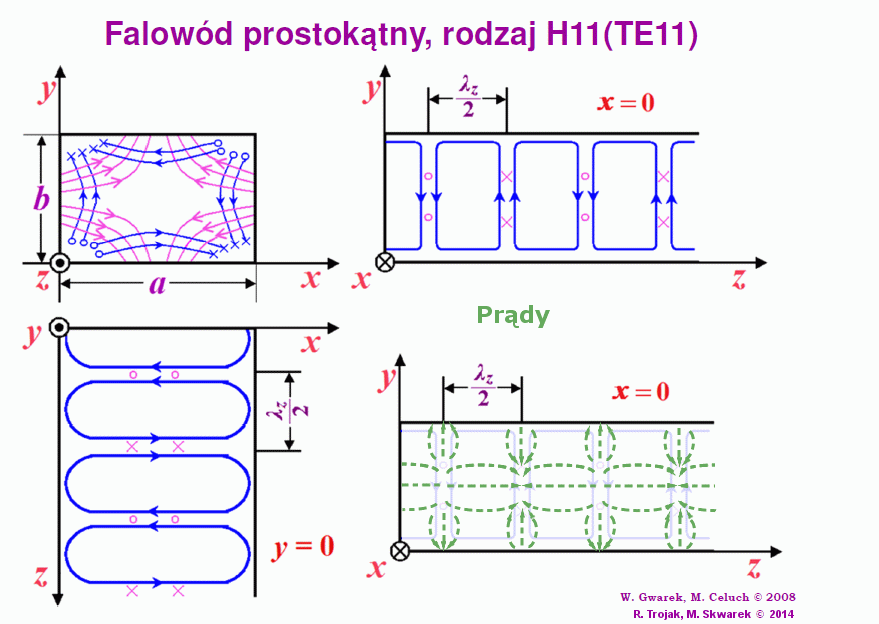
\includegraphics[scale=0.8]{4_1}$
	\end{center}


\item Rozkład pól dla fali stojącej 
	\begin{center}
	$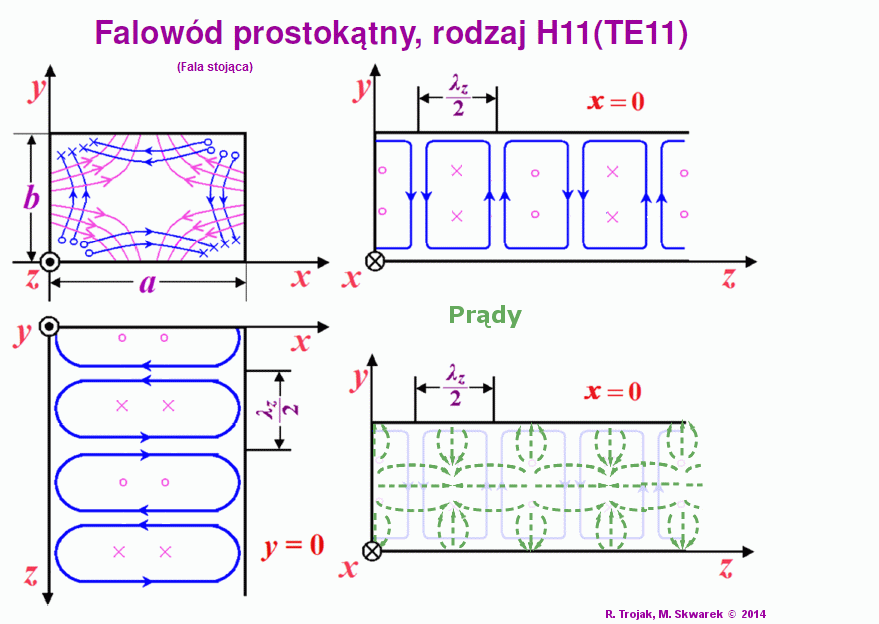
\includegraphics[scale=0.8]{4_2}$

	\end{center}

\end{enumerate}
\end{solution}
\section*{Zadanie 5.}
\begin{task}
Jakie są własności pół promieniowania dipola Hertza. Jak wykorzystuje się wzory na te pola w projektowaniu anten? Co to jest zysk kierunkowy anteny i jakie są metody jego powiększania? Zilustrować te metody na praktycznych przykładach kilku typów anten.\\
\end{task}

\begin{solution}

$$H\approx\vec{i_{\varphi}}\cfrac{I_{0}\beta l}{4\pi r}\sin{\theta}e^{j(\omega t-\beta r)}$$
$$E\approx\vec{i_{\theta}}\cfrac{I_{0}\beta^{2} l}{4\pi\epsilon\omega r}\sin{\theta}e^{j(\omega t-\beta r)}$$
Wyprowadzone między innymi z równań Maxwella.\\
Analizując powyższe wektory dowiadujemy się że:
\begin{itemize}
\item w dużej odległości od dipola Hertza, pole elektryczne i magnetyczne są do siebie prostopadłe, fazy są zgodne, a stosunek amplitud równy impedancji właściwej ośrodka.
\item wektor Poyntinga wynikający z istnienia pól jest zawsze skierowany wzdłuż wersora $\vec{i_{r}}$ co w połączeniu z wcześniejszymi cechami oznacza, że dipol Hertza jest źródłem promieniowania energii elektromagnetycznej.
\item pole elektyczne i magnetyczne w postaci wzorów opisują bezpośrednio gęstość mocy promieniowania dlatego nazwano je polami promieniowania
\item w dostatecznie malej odległości od dipola możemy przyjąć, energia pola magnetycznego jest pomijalnie mała w stosunku do energii pola elektrycznego.
\end{itemize}
\textbf{Zysk kierunkowy anteny}\\
Jest to stosunek mocy, jaką musiałaby wypromieniować izotropowa antena porównawcza, do mocy jaką promieniuje antena rozważana, jeśli gęstość mocy w tym samym kierunku ($\varphi,\ \theta$) i tej samej odległości są sobie równe.
$$G(\varphi,\ \theta)=\cfrac{p_i}{p}$$
\textbf{Związek parametrów anten z polami}\\
Niektóre własności oraz parametry można znaleźć dzięki wykorzystaniu wzorów na pole elektryczne oraz magnetyczne, np. do znalezienia charakterystyki promieniowania należy znaleźć najpierw pole magnetyczne w punkcie $P(r, \ \varphi,\ \theta)$ w strefie dalekiej od anteny. Pole to jest sumą pól dipoli elementarnych, z których składa się antena.\\
Zauważamy, że charakterystyką promieniowania możemy sterować za pomocą pola magnetycznego. Podobnie jest z innymi parametrami np. z rezystancją promieniowania, która wiąże się z mocą promieniowania obliczanej z wektora Poyntinga.
$$S(r,\ \varphi,\ \theta)=\cfrac{1}{2}E_{\theta}H_{\varphi}^{*}$$
Parametry, których wzory powiązane są ze wzorami pól mają wielką rolę dla projektujących anteny.\\

\textbf{Do uzyskania dużej kierunkowości stosujemy:}\\
\begin{itemize}
\item 'Ściany' antenowe a nawet prestrzenne rozmieszczenie dipoli
\item elektroniczne sterowanie amplitudy i fazy prądu
\item anteny z reflektorem
\item układy promieniujących szczelin w ściance falowodu
\end{itemize}

\end{solution}
\section*{Zadanie 6.}
\begin{task}
Omówić na czym polega efekt naskórkowy i jakie jest jego znaczenie w technice. Jak jest on zależny od częstotliwości? Srebro ma przewodność właściwą ok. $\sigma_{1}=6*10^{7} \big{[}\cfrac{S}{m}\big{]}$ a mosiądz ok. $\sigma_{2}=3*10^{7} \big{[}\cfrac{S}{m}\big{]}$. Zaproponować (i uzasadnić) jak grubą warstwą należy pokryć mosiężny falowód pracujący na częstotliwości 10GHz, aby uzyskać efekt zmniejszenia tłumienia przy stosunkowo małym koszcie.\\
\end{task}

\begin{solution}
\begin{itemize}
\item Efekt naskórkowy polega na tym, że kiedy fala elektromagnetyczna napotyka przewodnik, to wytwarza się na jego powierzchni prąd. Fale nie mogą wnikać w idealny przewodnik. Ładunki i prądy mogą istnieć tylko w nieskończenie cienkiej warstwie na powierzchni idealnego przewodnika.
\item Gdy przewodnik nie jest idealny, mówimy o głębokości wnikania $\delta=\cfrac{1}{\alpha}, \ \ \alpha\approx\sqrt{\frac{\omega\mu\sigma}{2}}$. Im większa częstotliwość, tym mniejsza głębokość wnikania i wtedy metal zachowuje się jak PEC.\\
\item Należy policzyć głębokość wnikania w srebrze przy 10 GHz. Srebro ma większą przewodność od mosiądzu, czyli wprowadza mniejsze tłumienie.
$$\delta_{w}=\cfrac{1}{\sqrt{\mu_{0}\sigma\pi}\sqrt{f}}=0.65 \big{[}\mu m\big{]}$$
\end{itemize}
\end{solution}
\section*{Zadanie 7.}
\begin{task}
Dana jest linia współosiowa o średnicy $7\ mm$ i średnicy wewnętrznej $3\ mm$ wykonana z miedzi o przewodności właściwej równej $5*10^{7}\ \cfrac{S}{m}$ i wypełniona dielektrykiem o przenikalności właściwej 2.00 i tangensie kąta stratności równym 0.002. Obliczyć parametry jednostkowe linii ($L_{1},\ C_{1},\ G_{1},\ R_{1}$) dla częstotliwości $1GHz$. Które (czy też który) z parametrów będzie wyraźnie różny dla częstotliwości $10GHz$. Ile razy stłumi się moc fali w tej linii na odcinku 10 m (dla $1\ GHz$ i dla $10\ GHz$).\\
\end{task}

\begin{solution}
\begin{center}
$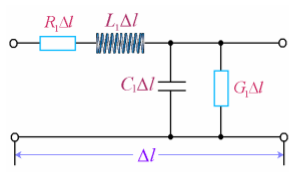
\includegraphics[scale=1]{7_1}$\\
\end{center}

$$L_{1}=\cfrac{\mu}{2\pi}\ln{\cfrac{a}{b}}=0.17\big{[}\cfrac{\mu H}{m}\big{]}$$
$$C_{1}=\cfrac{2\pi\epsilon}{\ln{\cfrac{a}{b}}}=0.13\big{[}\cfrac{nF}{m}\big{]}$$
$$\tg{\delta}=\cfrac{\sigma}{\omega\epsilon}=\cfrac{G_{1}}{\omega C_{1}} \ \ \implies \ G_{1}=\omega C_{1}\tg{\delta} = 0.82\big{[}\cfrac{mS}{m}\big{]}$$
$$\delta_{w}=\cfrac{2}{\sqrt{\omega\mu\sigma}}=2.25 \big{[}\mu m\big{]}$$
$$R=\cfrac{l}{\sigma S}\stackrel{l=1}{=}\cfrac{1}{\sigma S}\ \ \ S_{a}=2\pi a\delta_{w}\ \ \ S_{b}=2\pi b\delta_{w}$$
$$R_{1}=\cfrac{1}{ \sigma_{m}2 \pi a \detla_{w}}+\cfrac{1}{ \sigma_{m} 2 \pi \delta_{w}}=0.67 \big{[} \cfrac{\Omega}{m} \big{]}$$
$$\tg{\delta}=0.002=\cfrac{\sigma d}{\omega\epsilon}\ \ \implies \ \ \sigma d=\cfrac{4}{18}10^{-e}\big{[}\cfrac{S}{m}\big{]}$$
$$\alpha=\cfrac{\sigma d}{2}\sqrt{\cfrac{\mu}{\epsilon}}=\cfrac{10^{-3}}{9\sqrt{2}}$$
$$P(10m)=P(0)e^{-2\alpha 10m}\ \ \ \ \cfrac{P(10m)}{P(0m)}=e^{-2\alpha 10m}=0.553$$
\end{solution}

\section*{Zadanie 8.}
\begin{task}
Zdefiniować pojęcie dobroci rezonatora. Jaki jest sens fizyczny dobroci? Jakie znaczenie ma to pojęcie przy rozważaniu własności odwodów w dziedzinie częstotliwości i dziedzinie czasu? Do czego są wykorzystywane rezonatory? Jakie zalety ma zastosowanie rezonatorów dielektrycznych w miejsce rezonatorów wnękowych?\\
\end{task}

\begin{solution}
Dobroć jest współczynnikiem określającym stosunek średniej energii zgromadzonej w rezonatorze do średniej energii traconej w trakcie jednego okresu. //
Jest ona jednym z najważniejszych parametrów charakteryzujących właściwości rezonatora, wyraża się wzorem:
$$Q=2\pi\cfrac{\overline{W}}{\overline{P_{q}}T}$$
$\overline{W}$ - średnia energia magazynowana w rezonatorze\\
$\overline{P_{q}}$ - średnia moc strat w rezonatorze\\
$T$ - okres drgań\\

Warunek wystąpienia tlumienia aperiodycznego krytycznego jest równoważny zależności $Q=\cfrac{1}{2}$. Jeżeli dobroć rezonatora jest więszka niż $\cfrac{1}{2}$ to w rezonatorze jest możliwe wystąpienie oscylacji z pulsacją:
$$\omega_{v}^{'}=\omega\sqrt{1-\cfrac{1}{4Q^{2}}}$$
W rezonatorach o dużej dobroci pulsacja drgań własnych rezonatora nieznacznie różni się od pulsacji drgań własnych rezonatora bezstratnego $\omega_{v}$ dlatego często w zastosowaniach technicznych przyjmujemy, że: $\omega_{v}^{'}=\omega_{v}$. Oscylacje w rezonatorze są tłumione proporcjonalnie do finkcji $e^{-dt}$, gdzie $d$ jest współczynnikiem tłumienia wyrażającym się zależnością $d=\cfrac{\omega_{v}^{'}}{2Q}$. Jeżeli dobroć rezonatora jest nie większa niż $\cfrac{1}{2}$ to pole będzie tłumione bez oscylacji.\\
Rezonatory zbudowane z odcinków prowadnic falowych są najbardziej rozpowszechnione głównie dlatego, że można łatwo określić w nich rozkład pola, a więc łatwo można zaprojektować rezonator o zadanych parametrach.\\
Rezonator z przewodzącą ścianką o kształcie powierzchni kuli ma największą dobroć wśród rezonatorów o przewodzących ściankach, ze względu na optymalny stosunek objętości, w której gromadzi się energia do powierzchni niedoskonale przewodzących ścianek metalowych.\\
Zalety rezonatorów dielektrycznych względem wnękowych:
\begin{itemize}
\item mniejszy rozmiar i ciężar,
\item możliwość stosowania w różnych strukturach mikrofalowych i łatwy sposób sprzęgania z prowadnicami falowymi,
\item łatwy w przestrajaniu
\end{itemize}




\end{solution}
\section*{Zadanie 9.}
\begin{task}
Fala płaska biegnąca w kierunku $Ox$ i spolaryzowana liniowo tak, że pole elektryczne jest równoległe do osi $Oy$ i ma aplitudę $1\ \cfrac{V}{m}$ pada prostopadle na płytę doskonale przewodzącą, umieszczoną w płaszczyźnie $x=0$. Zapisać rzeczywistą postać wyrażeń na pole $E$ i $H$ dla fali padającej, odbitej i przechodzącej. Obliczyć gęstość powierzchniową prądu płynącego po płycie. Narysować obwiednie pola $E$ i $H$ w otoczeniu płyty. Wyjaśnić, co zmieni się, gdy płyta będzie miała przewodność właściwą $\sigma$ dużą, ale ograniczoną. Narysować obwiednie pól $E$ i $H$ w płycie dla dwóch różnych wartości $\sigma_{1}$ oraz $\sigma{2}=2\sigma_{1}$.\\
\end{task}

\begin{solution}
Postać rzeczywista \textsl{E} i \textsl{H}:
\begin{itemize}
\item $\vec{E^{+}_{1}}=\vec{i_{y}}cos(wt-\beta x)$\\
       $\vec{E^{-}_{1}}=-\vec{i_{y}}cos(wt+\beta x)$\\
       $\vec{E_{2}}=0$
\item $\vec{H^{+}_{1}}=\vec{i_{z}}\cfrac{1}{Z}cos(wt-\beta x)$\\
       $\vec{H^{-}_{1}}=\vec{i_{z}}\cfrac{1}{Z}cos(wt+\beta x)$\\
       $\vec{H_{2}}=0$\\
\end{itemize}
\textbf{Obliczanie gęstości prądu powierzchniowego:}\\
Z warunków brzegowych: $\vec{J_{s}}=\vec{n}\times(\vec{H_{2}}-\vec{H_1})\ \ \implies J_{s}=H_{0}=\cfrac{1}{Z}$

\begin{center}
Obwiednia pól $E$ i $H$ przy padaniu na idealny przewodnik:\\
$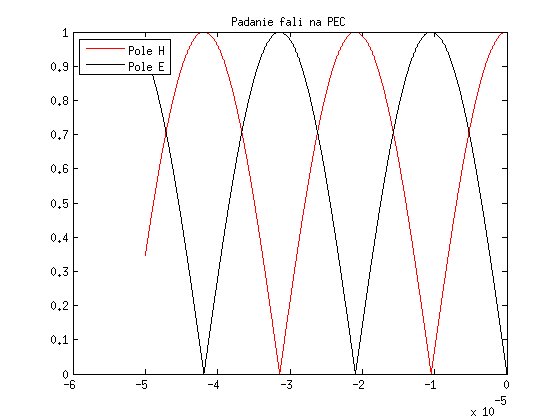
\includegraphics[scale=1]{9_1}$\\

$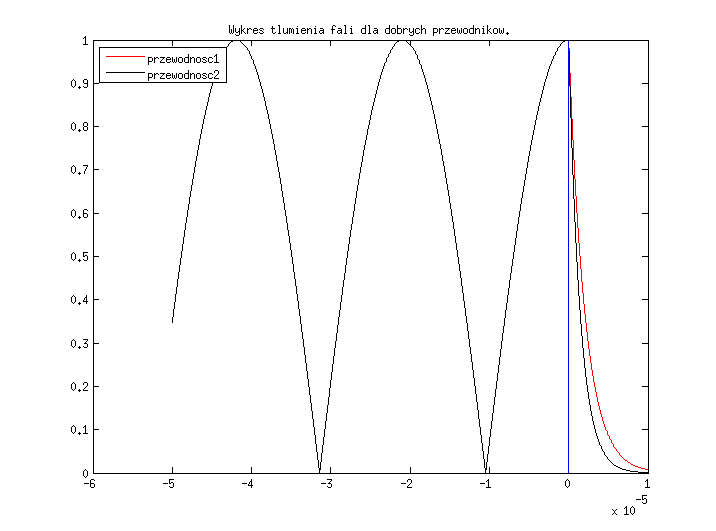
\includegraphics[scale=0.8]{9_2}$\\
\end{center}
Dla dużej ale nie nieskończonej $\sigma$ fale wejdą w przewodnik, ale zostaną bardzo szybko stłumione (skala na osi X na rysunku). Spowoduje to przepływ prądu po bardzo cienkiej powierzchni (ale nie nieskończenie cienkiej) $\rightarrow$ efekt naskórkowy.

\end{solution}

\section*{Zadanie 10.}
\begin{task}
Wymienić najczęściej stosowane w praktyce rodzaje linii TEM. Narysować (w przekrojach wzdłużnym i poprzecznym) rozkłady pól $E$ i $H$ dla rozchodzącej się w nich fali bieżącej. Podać cechy każdego z wymienionych typów linii determinujące ich zakres zastosowań praktycznych.\\
\end{task}

\begin{solution}
\begin{itemize}
\item Najczęściej stosowane linie TEM:
	\begin{itemize}
	\item linia współosiowa (najczęściej)
	\item symteryczna linia paskowa
	\item niesymetryczna linia paskowa (linia mikropaskowa, quasi-TEM)
	\item symetryczna linia dwuprzewodowa
	\end{itemize}
\item linia współosiowa - rozkład pól\\
$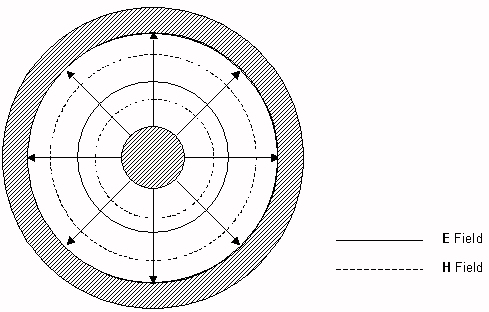
\includegraphics[scale=1.5]{10_1}$    $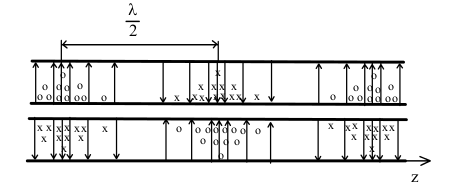
\includegraphics[scale=0.7]{10_2}$
\item symetryczna linia paskowa - rozkład pól\\
$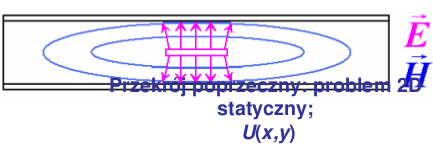
\includegraphics[scale=0.7]{22_2}$    $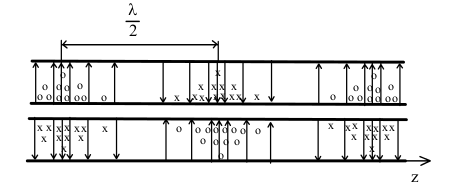
\includegraphics[scale=0.6]{10_2}$
\item niesymetryczna linia paskowa - rozkład pól\\
$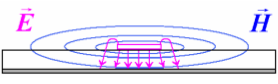
\includegraphics[scale=1]{10_3}$    $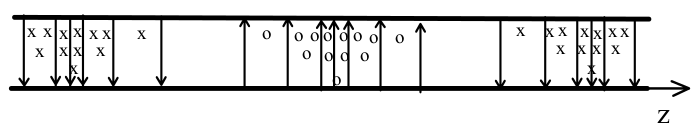
\includegraphics[scale=0.6]{35_2}$
\item Symetryczna linia dwuprzewodowa - rozkład pól\\
$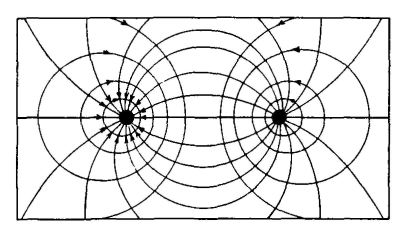
\includegraphics[scale=0.6]{10_4}$
\item Cechy linii współosiowej:
	\begin{itemize}
	\item dobre ekranowanie od pól zewnętrznych (na zewnątrz linie pola elektromagnetycznego są zerowe)
	\item ograniczony zakres impedancji charakterystycznych $Z_{c}=\cfrac{Z}{2\pi}\ln{\cfrac{a}{b}}$
	\item trudno robić rozgałęzienia oraz odcinki linii sprzężonych
	\item trudności z dołączaniem elementów skupionych
\end{itemize}
Typowe zakresy częstotliwości: kilkadziesiąt $MHz$ do kilku $GHz$. Czasami stosowana do niskich częstotliwości. Wynika to z faktu, że pola przesyłanej fali dla tej linii są dobrze odizolowane od pól zewnętrznych, a więc fala ta nie jest zakłócana z zewnątrz ani też nie zakłóca innych fal.

\item Cechy linii symetrycznej paskowej:\\ W stosunku do linii współosiowej znaacznie ułatwia budowanie rozgałęzień i linii sprzężonych. Stosowana do między innymi budowy filtów i sprzęgaczy mikrofalowych.\\
Przy odpowiednio szerokich płytach ekranujących (górnej i dolnej o jednakowym potencjale) możemy uznać, że pole, podobnie jak w linii współosiowej jest zamknięte wewnątrz linii, a więc dobrze odizolowane od otoczenia.

\item Cechy linii niesymetrycznej paskowej:
	\begin{itemize}
	\item łatwość w montowaniu elementów skupionych
	\item łatwośći przystosowania do masowej produkcji
	\item zależności długości fali od szerokości linii
	\item zależność parametrów od częstotliwości (dyspersja)
	\item gorsze odseparowanie od pól zewnętrznych oraz promieniowanie
	\end{itemize}
Zastosowanie: Powszechnie stosowana w układach analogowych, układach cyfrowych oraz układach scalonych
\item Cechy linii symetrycznej dwuprzewodowej:
	\begin{itemize}
	\item stosowana w energetyce
	\item stosowana do wysokich częstotliwości
	\item rozpraszanie pola na zewnątrz, sygnał przesyłany może sprzęgać się z innymi sygnałami
	\item prostota budowy
	\item możliwość realizacji linii o dużej impedancji charakterystycznej (rzędy kilkuset $\Omega$ )
	\item stosowana do połączenia odbiorników telewizyjnych z antenami
	\end{itemize}
\end{itemize}
\end{solution}
\section*{Zadanie 11.}
\begin{task}

Dane są rezonatory o ściankach idealnie przewodzących: 
\begin{enumerate}[a)]
\item Prostopadłościenny o wymiarach (podane kolejno w kierunki osi x,y i z) a = 3cm, b = 4cm i c = 10cm;
\item Cylindryczny o średnicy d = 10cm i wysokości h = 2cm.
\end{enumerate}
W każdym przypadku nazwać dwa rodzaje rezonansowe o najniższych częstosliwościach, obliczyć ich częstotliwości drgań własnych oraz naszkicować rozkłady pola elektrycznego w każdym z nich.\\

\end{task}


\begin{solution}
\begin{enumerate}[a)]

\item $\lambda_{rez} = \frac{2}{\sqrt{(\frac{m}{a})^2+(\frac{n}{b})^2+(\frac{p}{c})^2}} \\
f_{rez} = \frac{c}{\lambda_{rez}} \qquad$
$f_{rez} = \frac {c \cdot \sqrt{(\frac{m}{a})^2+(\frac{n}{b})^2+(\frac{p}{c})^2}}{2}$\\

Obliczenia dla rodzaju H (TE): \\
$f_{011} = \frac{3 \cdot 10^8}{2} \cdot \sqrt{(\frac{0}{0,03})^2+(\frac{1}{0,04})^2+(\frac{1}{0,1})^2} = 4038873605,351 Hz = \underline{4,04 GHz} $\\
$f_{101} = \frac{3 \cdot 10^8}{2} \cdot \sqrt{(\frac{1}{0,03})^2+(\frac{0}{0,04})^2+(\frac{1}{0,1})^2} = 5220153254,455 Hz = 5,22 GHz $\\
$f_{111} = \frac{3 \cdot 10^8}{2} \cdot \sqrt{(\frac{1}{0,03})^2+(\frac{1}{0,04})^2+(\frac{1}{0,1})^2} = 6427480066,091 Hz = 6,43 GHz$\\
\begin{center}
    $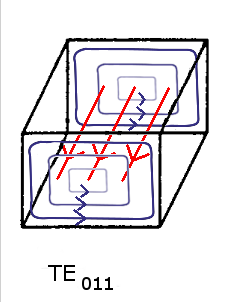
\includegraphics[scale=1]{11_1}$\\
\end{center}

Obliczenia dla rodzaju E (TM): \\

$f_{211} = \frac{3 \cdot 10^8}{2} \cdot \sqrt{(\frac{2}{0,03})^2+(\frac{1}{0,04})^2+(\frac{1}{0,1})^2} = 10784827305,062 Hz = 10,78 GHz $\\
$f_{111} = \frac{3 \cdot 10^8}{2} \cdot \sqrt{(\frac{1}{0,03})^2+(\frac{1}{0,04})^2+(\frac{1}{0,1})^2} = 6427480066,091 Hz =  \underline{6,43 Ghz}$\\
$f_{112} = \frac{3 \cdot 10^8}{2} \cdot \sqrt{(\frac{1}{0,03})^2+(\frac{1}{0,04})^2+(\frac{2}{0,1})^2} = 6932712311,931 Hz = 6,93 GHz $\\
$f_{121} = \frac{3 \cdot 10^8}{2} \cdot \sqrt{(\frac{1}{0,03})^2+(\frac{2}{0,04})^2+(\frac{1}{0,1})^2} = 9137833441,249 Hz = 9,15 GHz$\\
\begin{center}
    $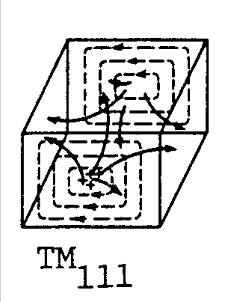
\includegraphics[scale=1]{11_2}$\\
\end{center}

\item W rezonatorze cylindrycznym warunki brzegowe uniemożliwiają utworzenie się rodzaju $H_{mn0} (TE_{mn0})$\\. \\
Pulsacja drgań własnych dla rodzaju H (TE): \\
 $\omega_v = \frac{1}{\sqrt{\mu \varepsilon}} \cdot \sqrt{(\frac{ \chi'_{mn} }{d})^2+(\frac{ \pi }{h})^2} $\\
$\omega_v = 2 \cdot \pi \cdot f_v$\\
$f_v = \frac{\omega_v}{2\cdot \pi} $\\
$f_v = \frac{1}{2\pi\sqrt{\mu \varepsilon}}\sqrt{(\frac{ \chi'_{mn} }{d})^2+(\frac{ \pi }{h})^2} $\\
$\sqrt{\mu_0 \varepsilon_0}=3,33 \cdot 10^{-9}$ \\

    \begin{center}
        $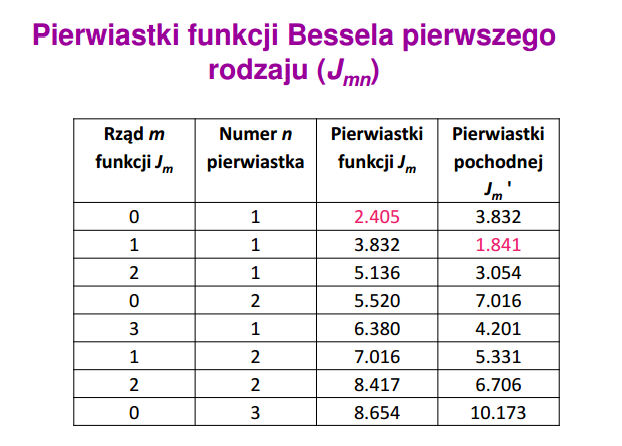
\includegraphics[scale=1]{11_bessel}$\\
    \end{center}

$f_{01p} = \frac{1}{2\pi \cdot 3,33 \cdot 10^{-9}}\sqrt{(\frac{ \chi'_{01} }{0,1})^2+(\frac{ \pi }{0,02})^2} = 7,72 GHz$\\
$f_{11p} = \frac{1}{2\pi \cdot 3,33 \cdot 10^{-9}}\sqrt{(\frac{ \chi'_{11} }{0,1})^2+(\frac{ \pi }{0,02})^2} = \underline{7,55 GHz}$\\
$f_{21p} = \frac{1}{2\pi \cdot 3,33 \cdot 10^{-9}}\sqrt{(\frac{ \chi'_{21} }{0,1})^2+(\frac{ \pi }{0,02})^2} = 7,64 GHz$\\
$f_{02p} = \frac{1}{2\pi \cdot 3,33 \cdot 10^{-9}}\sqrt{(\frac{ \chi'_{02} }{0,1})^2+(\frac{ \pi }{0,02})^2} = 8,21 GHz$\\
$f_{31p} = \frac{1}{2\pi \cdot 3,33 \cdot 10^{-9}}\sqrt{(\frac{ \chi'_{31} }{0,1})^2+(\frac{ \pi }{0,02})^2} = 7,76 GHz$\\
$f_{12p} = \frac{1}{2\pi \cdot 3,33 \cdot 10^{-9}}\sqrt{(\frac{ \chi'_{12} }{0,1})^2+(\frac{ \pi }{0,02})^2} = 7,92 GHz$\\
$f_{22p} = \frac{1}{2\pi \cdot 3,33 \cdot 10^{-9}}\sqrt{(\frac{ \chi'_{22} }{0,1})^2+(\frac{ \pi }{0,02})^2} = 8,16 GHz$\\
$f_{03p} = \frac{1}{2\pi \cdot 3,33 \cdot 10^{-9}}\sqrt{(\frac{ \chi'_{03} }{0,1})^2+(\frac{ \pi }{0,02})^2} = 8,93 GHz$\\

    \begin{center}
        $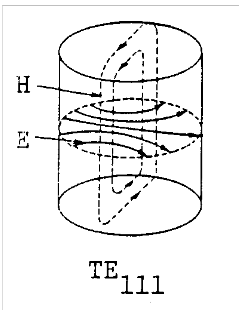
\includegraphics[scale=1]{11_3}$\\
    \end{center}

Dla rodzaju E w falowodzie $\beta_g = \frac{\chi_mn}{d}$ więc pulsacja drgań własnych pola rodzaju E wynosi \\
$f = \frac{1}{2\pi\sqrt{\mu \varepsilon}} \cdot \frac{\chi_{mn}}{d}$\\
$\sqrt{\mu_0 \varepsilon_0}=3,33 \cdot 10^{-9}$ \\
\\
$f_{01p} = \frac{1}{2\pi\sqrt{\mu \varepsilon}} \cdot \frac{\chi_{01}}{0,1} = \underline{1,15 GHz}$\\
$f_{11p} = \frac{1}{2\pi\sqrt{\mu \varepsilon}} \cdot \frac{\chi_{11}}{0,1} = 1,83 GHz$\\
$f_{21p} = \frac{1}{2\pi\sqrt{\mu \varepsilon}} \cdot \frac{\chi_{21}}{0,1} = 2,45 GHz$\\
$f_{02p} = \frac{1}{2\pi\sqrt{\mu \varepsilon}} \cdot \frac{\chi_{02}}{0,1} = 2,64 GHz$\\
$f_{31p} = \frac{1}{2\pi\sqrt{\mu \varepsilon}} \cdot \frac{\chi_{31}}{0,1} = 3,05 GHz$\\
$f_{12p} = \frac{1}{2\pi\sqrt{\mu \varepsilon}} \cdot \frac{\chi_{12}}{0,1} = 3,35 GHz$\\
$f_{22p} = \frac{1}{2\pi\sqrt{\mu \varepsilon}} \cdot \frac{\chi_{22}}{0,1} = 4,02 GHz$\\
$f_{03p} = \frac{1}{2\pi\sqrt{\mu \varepsilon}} \cdot \frac{\chi_{03}}{0,1} = 4,13 GHz$\\

    \begin{center}
        $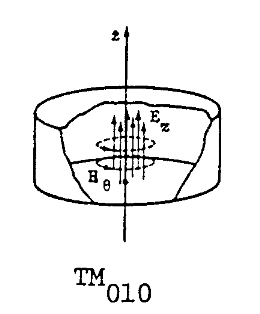
\includegraphics[scale=1]{11_4}$\\
    \end{center}
    \end{enumerate}
\end{solution}
\section*{Zadanie 12.}
\begin{task}
W próżni rozchodzi się w kierunku wersora $k$ o składowych $\big{(}\cfrac{1}{2},0,\cfrac{\sqrt{3}}{2}\big{)}$ fala płaska o polaryzacji kołowej (lewoskrętnej) i częstotliwości 30 MHz. Stwierdzono, że w punkcie (0,0,0) amplituda zespolona składowej pola magnetycznego skierowanej w kierunku osi $Oy$ wynosi $H_{y}=10j\ \big{[}\cfrac{A}{m}\big{]}.\\$
Podać pełne wyrażenie na rzeczywistą zależność od czasu pola elektrycznego w punkcie (1,1,1)[m].\\
Uwaga: Podać systematycznie w punktach drogę prowadzącą do rozwiązania.\\
\end{task}

\begin{solution}


$$\vec{k}=\big{[}\cfrac{1}{2};0;\cfrac{\sqrt{3}}{2}\big{]} \ \ \ f = 30 MHz \ \ \ H_{y}(0,0,0)=10j$$
Z własności rozchodzenia się fali płaskiej wynika, że: $\vec{k}\dot\vec{H}=0$, więc:
$$\vec{k}\circ\vec{H}=\cfrac{1}{2}H_{x}+\cfrac{\sqrt{3}}{2}H_{z}=0 \ \ \implies \ \ H_{x}=-\sqrt{3}H_{z}$$
Wiemy z polecenia, że polaryzacja fali ma być kołowa, co mówi nam, że składowe pola muszą być przesunięte o $\cfrac{\pi}{2}$ względem siebie. Jeżeli w punkcjie (0,0,0) mamy amplitudę urojoną, to druga składowa musi być rzeczywista, a więc pole $H$ można zapisać jako: $\vec{H}=\vec{H_{1}}+\vec{H_{2}}$. Z informacji, że mamy falę spolaryzowaną kołowo wnioskujemy, że amplitudy obu składowych są sobie równe:
$$|\vec{H_{1}}|=|\vec{H_{2}}| \ \ \stackrel{\substack{\vec{H_{1}}=10j \\ \vec{H_{2}}=H_{x}+H_{z}} }{\implies} \ \ 10=\sqrt{H_{x}^{2}+H_{z}^{2}}=\sqrt{3H_{z}^{2}+H_{z}^{2}}=2H_{z}$$
$$H_{z}=\stackrel{+}{-}5\ \ \ H_{x}=\stackrel{+}{-}5\sqrt{3}$$
Jeżeli polaryzacja ma być lewoskrętna, musi być spełniony warunek:\\
\begin{center} $ \vec{H_{2}} \times \vec{H_{1}} \parallel \vec{k} $, więc sprawdzamy:\\
\end{center}

\begin{itemize}
\item $\vec{H_{2}^{'}}\times\vec{H_{1}} = \begin{vmatrix}
					                    \vec{i_{x}}&\vec{i_{y}}&\vec{i_{z}}\\
					                    -5\sqrt{3}&0&5\\
					                    0&10&0\end{vmatrix} = -50\vec{i_{x}} -50\sqrt{3}\vec{i_{z}} \ \ \ \not\parallel \vec{k}$
					                    
\item $\vec{H_{2}^{''}}\times\vec{H_{1}} = \begin{vmatrix}
					                    \vec{i_{x}}&\vec{i_{y}}&\vec{i_{z}}\\
					                    5\sqrt{3}&0&-5\\
					                    0&10&0\end{vmatrix} = 50\vec{i_{x}} + 50\sqrt{3}\vec{i_{z}} \ \ \ \ \parallel \vec{k}$

\end{itemize}

Zatem ogólne wyrażenie na pole $\vec{H}$ w dowolnym punkcie wynosi:
$$ \vec{H_{re}} = \big{(} 5\sqrt{3}\vec{i_{x}}+5\vec{i_{z}}  \big{)}\cos{(\omega t - \beta \vec{k}\cdot\vec{r})} + 10\vec{i_{y}}\cos{(\omega t - \beta \vec{k}\cdot\vec{r}+\cfrac{\pi}{2}}) $$ $$ 
\vec{H_{re}} =\big{(}  5\sqrt{3}\vec{i_{x}}+5\vec{i_{z}} \big{)}\cos{(\omega t - \beta(\cfrac{1}{2}\vec{i_{x}}+\cfrac{\sqrt{3}}{2}\vec{i_{z}})\cdot (x\vec{i_{x}}+y\vec{i_{y}}+z\vec{i_{z}}) )} +$$ $$+ 10\vec{i_{y}}\cos{(\omega t - \beta(\cfrac{1}{2}\vec{i_{x}}+\cfrac{\sqrt{3}}{2}\vec{i_{z}})\cdot (x\vec{i_{x}}+y\vec{i_{y}}+z\vec{i_{z}})+\cfrac{\pi}{2} )}$$

Pole $\vec{E}$ obliczamy z własności fali płaskiej:
$$\vec{E}=Z(\vec{H}\times\vec{k})=Z H_{0} e^{j(\omega t - \beta\vec{k}\cdot\vec{r})}\begin{vmatrix}
					\vec{i_{x}}&\vec{i_{y}}&\vec{i_{z}}\\
				    5\sqrt{3}&10j&5\\
					\cfrac{1}{2}&0&\cfrac{\sqrt{3}}{2}\end{vmatrix}=Z H_{0} e^{j(\omega t           -        \beta\vec{k}\cdot\vec{r})}\big{(}5\sqrt{3}j\cdot\vec{i_{x}}-5j\cdot\vec{i_{z}}  \big{)}$$
Ogólne wyrażenie na pole $\vec{E}$ w dowolnej chwili i czasie wynosi:
$$\vec{E_{re}}= |Z| H_{0} \sin{(\omega t-\beta\vec{k}\cdot\vec{r}+Arg\ Z)}\big{(}-5\sqrt{3}\cdot\vec{i_{x}}+5\cdot\vec{i_{z}}  \big{)}$$
Zaś w punkcie (1,1,1):
$$ \vec{E}(1,1,1) = |Z| H_{0} \sin{(\omega t-\beta(\cfrac{1}{2}\vec{i_{x}}+\cfrac{\sqrt{3}}{2}\vec{i_{z}})\cdot (1\cdot\vec{i_{x}}+1\cdot\vec{i_{y}}+1\cdot\vec{i_{z}})+Arg\ Z)}\big{(}-5\sqrt{3}\cdot\vec{i_{x}}+5\cdot\vec{i_{z}}  \big{)}= $$
$\stackrel{\substack{Arg\ Z = 0 \\ \beta = \cfrac{\pi}{5}}}{=} 120\pi \cdot 10 \sin{\big{(}6\cdot 10^{7} t-\cfrac{\pi(1+\sqrt{3})}{10}\big{)}}\big{(}-5\sqrt{3}\cdot\vec{i_{x}}+5\cdot\vec{i_{z}}  \big{)}  $
\end{solution}
\section*{Zadanie 13.}
\begin{task}
Dany jest ośrodek o stałych $\mu,\ \epsilon,\ \sigma,$ w którym rozchodzi się płaska fala elektromagnetyczna. Narysować w skali podwójnie logarytmicznej wykresy współczynnika tłumienia oraz długości fali w funkcji częstotliwości. Jakie wnioski można stąd wyciągnąć odnośnie przesyłania fal radiowych w takich ośrodkach jak grunt czy woda morska? Zaznaczyć na wykresie obszar występowania efektu naskórkowego.\\
\end{task}

\begin{solution}


Zakładam, że dobry przewodnik, czyli: $\sigma=6*10^{7}\cfrac{S}{m}, \ \ \ \epsilon_{r}=\mu_{r}=1$.

\begin{center}
$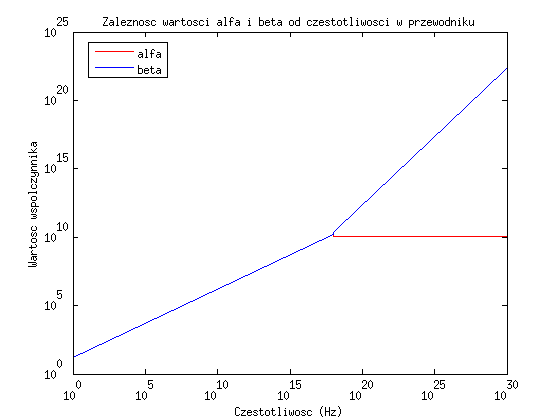
\includegraphics[scale=0.8]{13_1}$\\
\end{center}
\begin{center}
$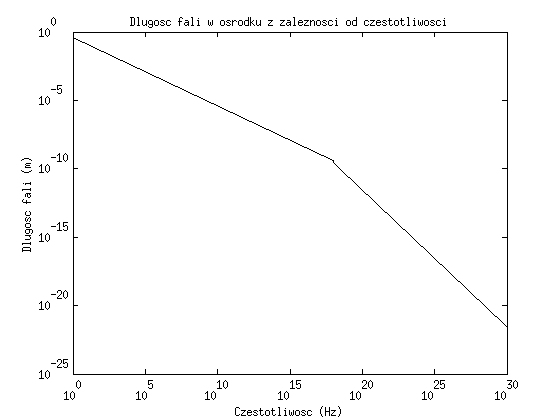
\includegraphics[scale=0.8]{13_2}$\\
\end{center}

Efekt naskórkowy występuje gdy $\alpha = \beta$, czyli w zakresie częstotliwości $10^{0} - 10^{18}$ Hz. Jednostki: $\alpha = \cfrac{1}{m}\ \ \ \beta=\cfrac{rad}{m}$.

\end{solution}
\section*{Zadanie 14.}
\begin{task}
Dany jest odcinek linii współosiowej(wypełnionej powietrzem) o średnicach przewodów 7 mm oraz 3.04 mm wykonanej z mosiądzu o przewodności właściwej $\sigma=3*10^{7} \cfrac{S}{m}$.
\begin{itemize}
\item Jaka będzie pojemność rozwartego odcinka linii o długości 10 cm?
\item O ile (w dB) stłumi się na tym odcinku fala bieżąca o częstotliwości $10\ GHz$?
\item Jak będzie się zmieniało to tłumienie ze zmianą częstotliwości?
\item Jaka będzie częstotliwość drgań własnych rodzaju podstawowego jeśli ten odcinek zostanie zwarty na obu końcach? Narysować rozkład prądów płynących w płytkach zwierających linie po obu stronach.\\
\end{itemize}
\end{task}

\begin{solution}
\begin{itemize}
\item pojemność linii 10m:\\
$$C=\cfrac{Q}{U} \ \ \ C_{1}=\cfrac{2\pi\epsilon}{\ln{\cfrac{a}{b}}}$$
$$C_{1}=\cfrac{2\pi10^{-9}\cfrac{1}{36\pi}}{\ln{\cfrac{7}{3.04}}}=1.53*10^{-10}\ F$$
$$C_{l=10m}=15.3\ pF$$

\item Tłumienie:\\
$\alpha\approx\cfrac{1}{2\omega}\big{(} \cfrac{R_{1}}{L_{1}} +\cfrac{G_{1}}{C_{1}} \big{)} \ \leftarrow \ \ $Wzór dostępny w książce przy budowie linii (strona ok. $160$)\\
$\sigma_{p}=3*10^{7} \cfrac{S}{m} \ \ \ \ \sigma_{d}=0$ przewodności (odpowiednio przewodników i dielektryka)\\
$\delta_{w}=\sqrt{\cfrac{2}{\omega\mu\sigma_{p}}}\ \leftarrow \ \ $ głębokość wnikania\\
$$G_{1}=\cfrac{2\pi\sigma_{d}}{\ln{\cfrac{a}{b}}}\ \ \ R_{1}=\cfrac{1}{2\pi\sigma_{p}\delta_{w}}\big{(} \cfrac{1}{a} + \cfrac{1}{b} \big{)} \ \ \ L_{1} = \cfrac{\mu}{2\pi}\ln{\cfrac{a}{b}}$$
\item Wraz ze wzrostem częstotliwości tłumienie maleje.
\item $f_{r}=\cfrac{c}{2l} \ \ \ l=\cfrac{\lambda_{r}}{2} \ \ \ f_{r}=\cfrac{3*10^{8}}{2*0.1}=1.5\ GHz$\\
Rozkłady pól:
\begin{center}
$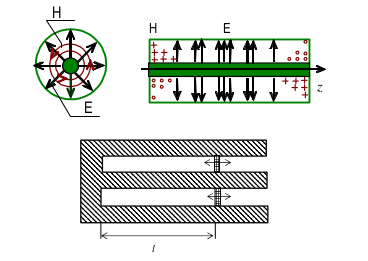
\includegraphics[scale=1]{14}$\\
\end{center}
\end{itemize}
\end{solution}
\section*{Zadanie 15.}
\begin{task}
Porównać (w zwięźle sformułowanych punktach) ogólne własności fal TEM w liniach przesyłowych oraz \textsl{E}
i \textsl{H} w falowodach pod względem: (częstotliwości granicznej, definicji parametrów obwodowych, zmiennośći
parametrów w funkcji częstotliwości, prędkości fazowej i grupowej, wielorodzajowości).\\
\end{task}

\begin{solution}

\begin{itemize}
\item Częstotliwość graniczna:
    \begin{itemize}
    \item dla TEM 0 Hz w linii współosiowej
    \item dla falowodów zależy od rodzaju fali jaki się rozchodzi
        $$w_{g}=\sqrt{\cfrac{(\cfrac{m\pi}{a})^{2} + (\cfrac{n\pi}{b})^{2}}{\mu\epsilon}} $$
        \begin{itemize}
        \item $f<f_{g}$ - fala się nie rozchodzi (tłumiona)
        \item $f>f_{g}$ - fala się rozchodzi
        \end{itemize}
    \end{itemize}
\item parametry obwodowe
    \begin{itemize}
        \item TEM 
        \begin{itemize}
            \item maksymalne napięcie między przewodami:
                $U= \int_{b}^{a}E_{0}\cfrac{b}{\rho}d\rho$
            \item maksymalna wartość prądu w przewodach:
                $I=\oint_{l}\vec{H}d\vec{l}=\cfrac{\epsilon_{0}}{Z}2\pi b $
            \item impedancja charakterystyncza: 
                $Z_{c}=\cfrac{Z_{0}}{2\pi}\ln{\cfrac{a}{b}} $  
            \item pojemność jednostkowa:
                $C_{1}=\cfrac{q_{1}}{U}=\cfrac{2\pi\epsilon}{\ln{\cfrac{a}{b}}} $
            \item indukcyjność jednostkowa:
                $L_{1}=\cfrac{\mu}{2\pi}\ln{\cfrac{a}{b}} $
            \end{itemize}
          \item falowód 
            \begin{itemize} 
                \item impedancja charakterystyczna:
                $Z_{CUI}=\cfrac{U}{I}$$ $$Z_{CPU}=\cfrac{U^2}{2P}$, 
                $Z_{CPI}=\cfrac{2P}{I^2}$
                \item współczynnik propagacji: $\gamma_{z}=\sqrt{\beta_{g}^{2}-\beta^{2}}$
                \item $\beta_{z}=\beta\sqrt{1-\cfrac{\beta_{g}^{2}}{\beta}}$
                \item graniczna długość fali: $\lambda_{g}=\cfrac{2\pi}{\beta_{g}}=\cfrac{2}{\sqrt{(\cfrac{m}{a})^{2}+(\cfrac{n}{b})^{2}}} $
                \item długość fali w falowodzie:
                     $\lambda_{z}=\cfrac{2\pi}{\beta_{z}}=\cfrac{\lambda}{\sqrt{1-(\cfrac{\lambda}{\lambda_{g}})^{2}}} $            
                \item impedancja falowa dla fali typu E:
                     $Z_{f}=Z\sqrt{1-(\cfrac{\omega_{g}}{\omega})^{2}} $
                \item impedancja falowa dla fali typu H:
                    $Z_{f}=\cfrac{Z}{\sqrt{1-(\cfrac{\omega_{g}}{\omega})^{2}}} $
            \end{itemize} 
    \end{itemize}
\item zmienność parametrów w funkcji częstotliwości:
    \begin{itemize}
    \item TEM - od częstotliwości zależy współczynnik propagacji fali $\gamma=j\omega\sqrt{L_{1}C_{1}}$. 
            Wraz ze wzrostem częstotliwości wzrasta współczynnik propagacji.
    \item falowód - $\gamma_{z}$, $\beta_{z}$, $\lambda_z$, $Z_{f}$ zależą od częstotliwości      
    \end{itemize}
\item prędkość fazowa i grupowa
    \begin{itemize}
    \item dla fali tem TEM: $v_{g} = v_{f}$
    \item w falowodach prędkości są różne: $$v_{f}=\cfrac{V}{\sqrt{1-(\cfrac{\omega_{g}}{\omega})^2}} $$  
            $$v_{g}=v\sqrt{1-(\cfrac{\omega_{g}}{\omega})^{2}} $$
    \end{itemize}
\item wielorodzajowość
    \begin{itemize}
    \item w linii TEM zwykle jeden rodzaj, ale dla bardzo dużych częstotliwości można wzbudzić wyższe rodzaje
    \item w falowodzie  rodzaj zależy od wymiarów falowodu, można mieć jednocześnie kilka rodzajów. W falowodzie
            prostokątnym, wśród fal typu \textsl{E} podstawowym rodzajem jest $E_{11}$. Rodzaj ten ma największą
            wartość długości fali wśród rodzajów typu $E$.\\
            W zbiorze WSZYSTKICH rodzajów fal w falowodzie prostokątnym, podstawowym jest rodzaj $H_{10}$.    
    \end{itemize}
\end{itemize}

\end{solution}

\section*{Zadanie 16.}
\begin{task}
Narysować rozkład pól $E$ i $H$, wektora Poyntinga oraz prądów przewodzenia i przesunięcia w dwóch prostopadłych do siebie przekrojach wzdłużnych falowodu kołowego z falą A) bieżącą B) stojącą, rodzaju $E_{11}$. Opisać  jak będą się zmieniały te pola w funkcji czasu.\\
\end{task}

\begin{solution}

\begin{itemize}
	\item Fala bieżąca:
	\begin{center}
	$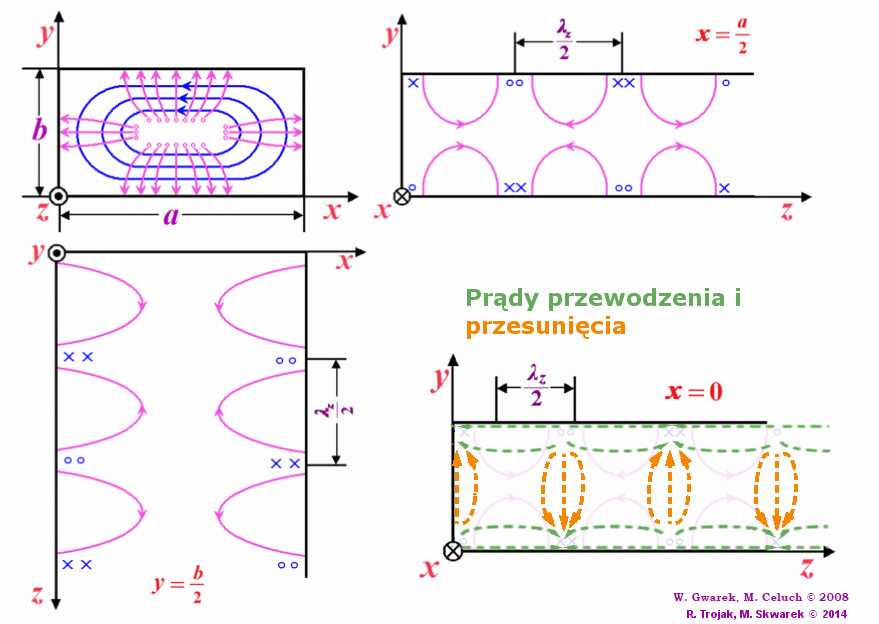
\includegraphics[scale=0.7]{16_1}$\\
	\end{center}
	\item Fala stojąca:\\
	
	
	\begin{center}
	$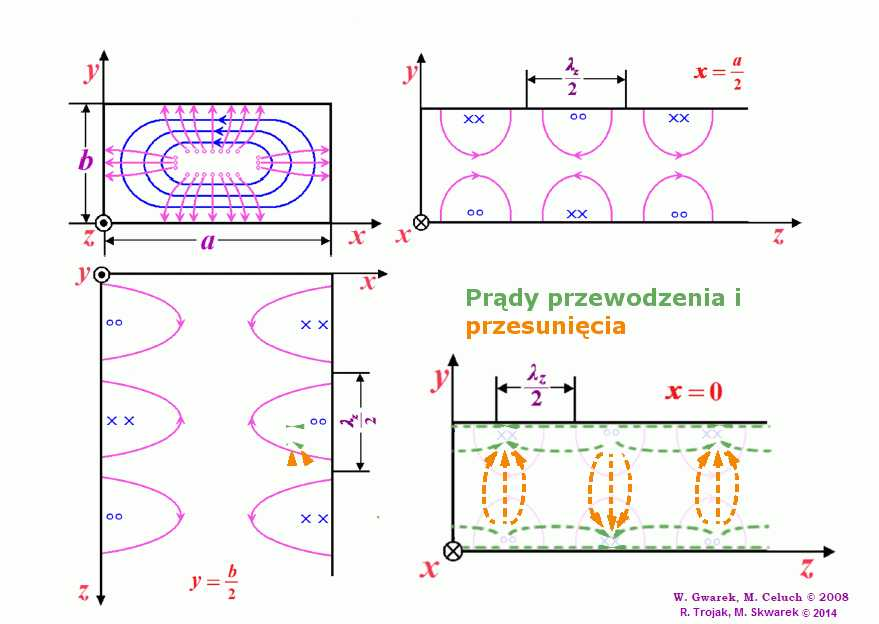
\includegraphics[scale=0.7]{16_2}$\\
	\end{center}
\end{itemize}
\end{solution}
\section*{Zadanie 17.}
\begin{task}
Przedyskutować fizyczne implikacje prawa Ampera w różnych przypadkach.\\
\end{task}

\begin{solution}
Drugie równanie Maxwella otrzymujemy z prawa Ampere`a mówiącego o związku między przepływającym prądem a polem magnetycznym wytwarzanym przez ten prąd. Prawo to ma następującą postać:
$$\oint_{l}\vec{H}d\vec{l}=I=\iint_{s}\vec{J}\vec{n}ds$$
$$\vec{J}=\vec{J_{d}}+\vec{J_{p}}+\vec{J_{u}}$$\\
$\vec{J_{p}}=\sigma\vec{E}$; $\vec{J_{u}}=\rho\vec{V}$; $\vec{J_{p}}$ - prąd przesunięcia.\\
Do wyrażenia określającego gęstość prądu przesunięcia możemy dojść rozważając proces ładowania lub rozładowywania kondensatora płaskiego. W czasie ładowania kondensatora do jego okładek dopływa prąd $I=\cfrac{dq}{dt}$. Między okładkami nie ma ładunków, prawo ciągłości prądu nie jest spełnione, dopóki nie założymy, że między okładkami kondensatora płynie także prąd o takiej samej wartości co w przewodach podłączonych do okładek, związany ze zmianami wektora indukcji elektrycznej w czasie ładowania kondensatora.\\

\begin{center}
$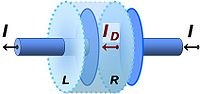
\includegraphics[scale=0.7]{17}$\\
\end{center}

$$\vec{J_{d}}=\cfrac{\partial\vec{D}}{\partial t}$$
Po sprowadzeniu gęstości prądu przesunięcia do prawa Ampere`a otrzymamy II równanie Maxwella w postaci całkowej:
$$\oint_{l}\vec{H}d\vec{l}=\iint(\vec{J}+\cfrac{\partial\vec{D}}{\partial t})\vec{n}ds, \ \vec{J}=\vec{J_{p}}+\vec{J_{u}}$$
Postać różniczkowa: $\nabla\times\vec{H}=\vec{J}$


\end{solution}


\section*{Zadanie 18.}
\begin{task}
Zdefiniować i zinterpretować (na wybranym przykładzie fizycznym) pojęcie źródłowości pola.\\
\end{task}

\begin{solution}
\textbf{Tutaj nie jestem pewien rozwiązania, bo zwyczajnie nie mogłem odczytać (szczególnie koniec).}\\
Dywergencję dowolnego wektora $\vec{A}$ możemy, na podstawie twierdzenia Gaussa, przedstawić w postaci:
$$\nabla\vec{A}=\lim_{V\to 0}\cfrac{\oiint\vec{A}d\vec{s}}{V}$$
$\oiint\vec{A}d\vec{s}$ - strumień wektora $\vec{A}$ wypływajcego z obszaru o objętości $V$. Dywergencja stanowi stosunek tego strumienia do objętości bardzo malego obszaru. Jeżeli w rozważanym punkcie przestrzeni znajduje się źródł skalarne pola $\vec{A}$ to stosunek ten jest różny od zera i punkt taki nazywany jest polem źródłowym. Jeżeli natomiast dywergencja pola $\vec{A}$ jest równa zero, mówimy o polu bezźródłowym.\\
\begin{center}
$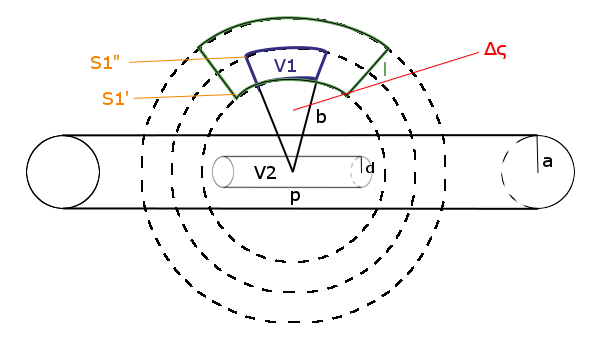
\includegraphics[scale=1]{18_1}$\\
\end{center}
Nieskończenie długi walec o promieniu $a$ naładowany jednoimiennym ładunkiem elektrycznym o gęstości objętościowej $\rho_{V}$.
$$\oiint_{S}\vec{D}\vec{n}ds=\iiint_{V}\rho_{V}dV$$
$$\vec{D}=\vec{i_{\rho}}\cfrac{\rho_{V}\rho}{a},\ \ \rho <a$$
$$\vec{D}=\vec{i_{\rho}}\cfrac{\rho_{V}a^{2}}{2},\ \ \rho >a$$\\ $\rho$ - współrzędne rozważanego punktu w przestrzeni w cylindrycznym układzie współrzędnych.\\
Strumień wektora $\vec{D}$ przepływający przez powierzchnię $S_{1}$ otaczamy obszarem $V_{1}$. Strumień wektora $\vec{D}$ różny od zera przeplywa jedynie przez ścianki $S_{1}^{'} i S_{1}^{''}$. $\vec{D}$ jest równolegly do pozostałych ścianek.
$$\oiint_{S_{1}}\vec{D}d\vec{s}=\oiint_{S{1}^{'}}\vec{D}d\vec{s}+\oiint_{S{1}^{''}}\vec{D}d\vec{s}=
\cfrac{\rho_{V}a^{2}pb\Delta\varphi}{2b} - \cfrac{\rho_{V}a^{2}p(b+l)\Delta\varphi}{2(b+l)}=0$$
Strumień $\vec{D}$ przepływający przez $S_{1}=0$. Pole $\vec{D}$ wytwarzane jest poza obszarem $V_{1}$, przenika przez jego granicę, ale strumień wpływający jest równy strumieniowi wypływającemu. Powoduje to, że pole $\vec{D}$ w $V_{1}$ spełnia $\nabla\vec{D}=0$. Przez mały walec o promieniu $d$, który leży na osi naładowanego cylindra nie przepływa żaden strumień wektora $\vec{D}$, więc możemy rozpatrywać tylko powierzchnię boczną.\\
$\vec{D}$ wypływa z walca przez całą powierzchnię, więc jest zawsze dodatni:
$$\oiint_{S_{2}}\vec{D}d\vec{s}=\cfrac{\rho_{v}d2\pi dp}{2}=\rho_{v}\pi d^{2}p$$
$$\cfrac{\oiint\vec{D}d\vec{s}}{V_{2}}=\cfrac{\rho_{v}\pi d^{2}p}{\pi d^{2}p}=\rho_{v}$$
W obszarze, w którym istnieje niezerowa gęstość objętności ładunków, pole indukcji elektrycznej jest źródłowe, a wartość dywergencji równa się gęstości objętościowej ładunku elektrycznego stanowiącego źródło skalarne tego pola.


\end{solution}
\section*{Zadanie 19.}
\begin{task}
Zespolony wektor pola elektrycznego fali o $f=1 GHz$ rozchodzącej się w ośrodku stratnym, o parametrach: $\mu=\mu_{0} \ \epsilon=\epsilon_{0}$, oraz impedancji właściwej $Z=|Z|e^{j\cfrac{\pi}{18}}$ wyraża się zależnością: $\vec{E}=(\vec{i_{x}}+3j\vec{i_{y}})e^{j(\omega t - \beta z) - \alpha z} [\cfrac{V}{m}]$.
\begin{enumerate}[a)]
\item Zapisać odpowiadający mu wektor $\vec{H}$ w postaci rzeczywistej oraz narysować krzywą zakreślaną przez koniec tego wektora w płaszczyźnie $0xy\ (z=0)$
\item Obliczyć wartości $|Z|$, $\alpha$ oraz $\beta$. Podać wzór na zależność od czasu wartości powierzchniowej gęstości mocy tej fali w płaszczyźnie $z=2m$. 
\end{enumerate}
\textbf{Uwaga: Można wybrać (po uprzednim zaznaczeniu) łatwiejszą wersję zadania z założeniem
ośrodka bezstratnego (Z rzeczywiste, $\alpha=0$) z oceną maksymalną 10 p.}\\
\end{task}

\begin{solution}
$$\vec{E}=(\vec{i_{x}}+3j\vec{i_{y}})e^{j(\omega t - \beta z)- \alpha z}$$
$$\vec{E}(t)=\vec{i_{x}}e^{-\alpha z}\cos(\omega t - \beta z)-3\vec{i_{y}}e^{-\alpha z}sin(\omega t - \beta z)$$
$$\vec{H}=\cfrac{\vec{k}\times\vec{E}}{Z}$$
\begin{enumerate}[a)]
\item $$\vec{H}(t)=\vec{i_{y}}\cfrac{1}{|Z|}e^{-\alpha z}\cos{(\omega t - \beta z + Arg Z)+\cfrac{3}{|Z|}\vec{i_{x}}e^{-\alpha z}sin(\omega t - \beta z + Arg Z)}$$\\
Wartości liczbowe mogą się troche różnić, ale ogólny sens obrazka jest zachowany (9902 to liczba punktów dla których rysowany był wykres). Oczywiście elipsa powinna być wyciągnięta w górę, o czym mówią wartości, ale jak się narysowało każdy widzi.
\begin{center}
$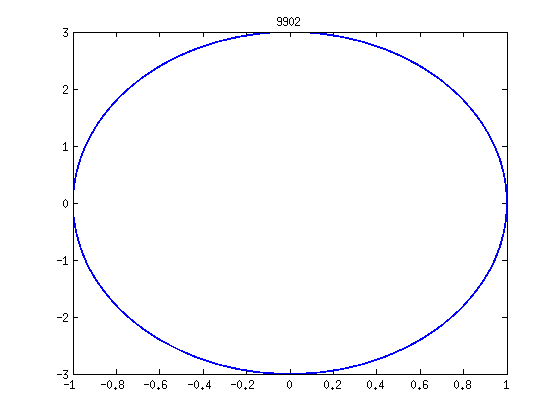
\includegraphics[scale=0.7]{19}$\\
\end{center}
\item $$Z=|Z|e^{j\cfrac{\pi}{18}}$$\\
$$Z=\sqrt{\cfrac{j\omega \mu}{\sigma + j\omega\epsilon}}=\sqrt{\cfrac{j\mu}{(\tg{\delta}+j)\epsilon}}=Z_{0}\sqrt{\cfrac{j}{\tg{\delta}+j}}$$
$$\delta = 2Arg Z\ \implies \delta = \cfrac{\pi}{9} \implies \tg{\delta}=0.35$$
$$|Z|=120\pi|\sqrt{\cfrac{j}{0.35+j}}|=365.7 \Omega$$
$$\gamma= \sqrt{j \omega\mu( \sigma+j \omega \epsilon)} = j \omega \sqrt{ \mu\eps} \big{(} 1 - j \cfrac{1}{2} \tg{ \delta}  \big{)} = 
2\cdot 10^{9}j\sqrt{\cfrac{1}{36\pi}\cdot 10^{-9}\cdot 4\pi\cdot 10^{-7}}\big{(} 1-\cfrac{1}{2}j\cdot 0.35 \big{)}=1.1(6)+ 6.(6)j$$\\
$\alpha=0.58(3) \ \cfrac{Np}{m}\\ \beta=3.(3)\ \cfrac{rad}{m} $\\
Wektor Poyntinga:
$$\vec{S}=\vec{E}\times\vec{H} =\cfrac{e^{-2\alpha x}}{|Z|} \begin{vmatrix}
					\vec{i_{x}}&\vec{i_{y}}&\vec{i_{z}}\\
					\cos{(\omega t-\beta z)}&-3\sin{(\omega t-\beta z+\cfrac{\pi}{18})}&0\\
					3\sin(\omega t - \beta z)&-\cos(\omega t - \beta z+\cfrac{\pi}{18})&0\end{vmatrix}=\cfrac{e^{-2\alpha x}}{|Z|} \big{(} \vec{i_{z}}\cos{(\omega t -\beta z)}\cos{(\omega t -\beta z + \cfrac{pi}{18})}+$$  $\ \ \ \ +\ \vec{i_{z}} 9\sin{(\omega t - \beta z)}\sin{(\omega t - \beta z+\cfrac{\pi}{18})} \big{)} $\\
$ \vec{S}(z=2m)=\cfrac{e^{-2.(3) x}}{365.7} \big{(} \vec{i_{z}}\cos{(2\cdot 10^{9} \pi t -13.(3))}\cos{(2\cdot 10^{9} \pi t -13.(3) + \cfrac{pi}{18})}+$\\ $\hspace{2.5cm} +\vec{i_{z}} 9\sin{(2\cdot 10^{9} \pi t - 13.(3))}\sin{(\omega t - 13.(3) +\cfrac{\pi}{18})} \big{)} $

\end{enumerate}
\end{solution}

\section*{Zadanie 20.}
\begin{task}
Zapisać w postaci rzeczywistej wektor pola elektrycznego i magnetycznego fali płaskiej o polaryzacji kołowej prawoskrętnej, rozchodzącej się w próżni w kierunku wersora \textbf{k} o składowych $\big{(}-\cfrac{1}{2},0,\cfrac{\sqrt{3}}{2}  \big{)}$ jeśli wiadomo, że w chwili t=0, w środku układu współrzędnych pole magnetyczne jest równoległe do osi Oy.\\
\end{task}

\begin{solution}


$$\vec{k}=\big{[}-\cfrac{1}{2};0;\cfrac{\sqrt{3}}{2}\big{]} $$
Z własności rozchodzenia się fali płaskiej wynika, że: $\vec{k}\cdot\vec{H}=0$, więc:
$$\vec{k}\cdot\vec{H}=-\cfrac{1}{2}H_{x}+\cfrac{\sqrt{3}}{2}H_{z}=0 \ \ \implies \ \ H_{x}=\sqrt{3}H_{z}$$
Wiemy z polecenia, że polaryzacja fali ma być kołowa, co mówi nam, że składowe pola muszą być przesunięte o $\cfrac{\pi}{2}$ względem siebie. Jeżeli w punkcie (0,0,0) mamy amplitudę rzeczywistą, to druga składowa musi być urojona, a więc pole $H$ można zapisać jako: $\vec{H}=\vec{H_{1}}+\vec{H_{2}}$. Z informacji, że mamy falę spolaryzowaną kołowo wnioskujemy, że amplitudy obu składowych są sobie równe:
$$|\vec{H_{1}}|=|\vec{H_{2}}| \ \ \implies \ \ H_{y}=\sqrt{H_{x}^{2}+H_{z}^{2}}=\sqrt{3H_{z}^{2}+H_{z}^{2}}=2H_{z}$$
$$H_{y}=\stackrel{+}{-}2H_{z}\ \ \ H_{x}=\stackrel{+}{-}2\sqrt{3}H_{z}$$
Wynika z tego, że zadania wymaga rozpatrzenia dwóch przypadków:\\
\begin{enumerate}[1*]
\item $\vec{H^{'}} = H_{z} e^{j(\omega t - \beta \vec{k} \cdot\vec{r})}\big{(} 2\sqrt{3}j\vec{i_{x}} + 2\vec{i_{y}} +j\vec{i_{z}} \big{)}$
\item $\vec{H^{''}} = H_{z} e^{j(\omega t - \beta \vec{k} \cdot\vec{r})}\big{(} -2\sqrt{3}j\vec{i_{x}} - 2\vec{i_{y}} +j\vec{i_{z}} \big{)}$
\end{enumerate}
Korzystamy z własności fali płaskiej:
$$ \vec{E} = \cfrac{\vec{H}\times\vec{k}}{Z} $$\\

\begin{enumerate}[1*]
\item $\vec{E_{1}}=\cfrac{\vec{H^{'}}\times\vec{k}}{Z} = \cfrac{H_{z}}{Z} e^{j(\omega t - \beta\vec{k} \cdot\vec{r})}          \begin{vmatrix}				                                                             \vec{i_{x}}&\vec{i_{y}}&\vec{i_{z}}\\
					                    2\sqrt{3}j&2&j\\
					                    -\cfrac{1}{2}&0&\cfrac{\sqrt{3}}{2}\end{vmatrix} = \cfrac{H_{z}}{Z} e^{j(\omega t - \beta\vec{k} \cdot\vec{r})}\big{(}\sqrt{3}\vec{i_{x}}+\cfrac{5}{2}j\vec{i_{y}} +\vec{i_{z}}\big{)}\\
\vec{E_{1}}=\cfrac{H_{z}}{Z} e^{j(\omega t - \beta\vec{k}\cdot\vec{r})}\big{(}\sqrt{3}\vec{i_{x}}+\vec{i_{z}}\big{)} + \cfrac{H_{z}}{Z} e^{j(\omega t - \beta\vec{k}\cdot\vec{r}+\cfrac{\pi}{2})}\cfrac{5}{2}\vec{i_{y}}\\
\vec{E_{1}}_{re} =\cfrac{H_{z}}{Z}\big{(} (\sqrt{3}\vec{i_{x}}+\vec{i_{z}})\cos{(\omega t - \beta\vec{k}\cdot\vec{r})} - \cfrac{5}{2}\vec{i_{y}}\sin{(\omega t - \beta\vec{k}\cdot\vec{r})}  \big{)} $
					      
					                    
\item $\vec{E_{2}}=\cfrac{\vec{H^{''}}\times\vec{k}}{Z} =\cfrac{H_{z}}{Z} e^{j(\omega t - \beta\vec{k} \cdot\vec{r})}           \begin{vmatrix}
					                    \vec{i_{x}}&\vec{i_{y}}&\vec{i_{z}}\\
					                    -2\sqrt{3}j&-2&j\\
					                    -\cfrac{1}{2}&0&\cfrac{\sqrt{3}}{2}\end{vmatrix} = \cfrac{H_{z}}{Z} e^{j(\omega t - \beta\vec{k} \cdot\vec{r})}\big{(}-\sqrt{3}\vec{i_{x}}+\cfrac{5}{2}j\vec{i_{y}} -\vec{i_{z}}\big{)}\\
\vec{E_{2}}=\cfrac{H_{z}}{Z} e^{j(\omega t - \beta\vec{k}\cdot\vec{r})}\big{(}-\sqrt{3}\vec{i_{x}}-\vec{i_{z}}\big{)} + \cfrac{H_{z}}{Z} e^{j(\omega t - \beta\vec{k}\cdot\vec{r}+\cfrac{\pi}{2})}\cfrac{5}{2}\vec{i_{y}}\\
\vec{E_{2}}_{re} =\cfrac{H_{z}}{Z}\big{(} -(\sqrt{3}\vec{i_{x}}+\vec{i_{z}})\cos{(\omega t - \beta\vec{k}\cdot\vec{r})} - \cfrac{5}{2}\vec{i_{y}}\sin{(\omega t - \beta\vec{k}\cdot\vec{r})}  \big{)}					                    
					                   $\\
\end{enumerate}
Polaryzację prawoskrętną mogą opisywać dwa wyrażenia:
$$ \vec{E} = \vec{i_{x}}E_{r}cos{(\omega t)} + \vec{i_{y}}E_{r}sin{(\omega t)} \ \ \ \vee\ \ \ 
    \vec{E} = -\vec{i_{x}}E_{r}sin{(\omega t)} + \vec{i_{y}}E_{r}cos{(\omega t)}$$\\
W naszym zadaniu przypadek 2* pasuje do pierwszego wyrażenia (wystarczy wyłączyć - przed nawias).\\
Więc ostatecznie odpowiedź do zadania:\\
$ \vec{H}_{re} = H_{z}\big{(} (-2\sqrt{3}\vec{i_{x}}+ \vec{i_{z}})\sin{(\omega t - \beta \vec{k} \cdot\vec{r})} - 2\vec{i_{y}}\cos{(\omega t - \beta \vec{k} \cdot\vec{r})} \big{)} $ 

$ \vec{E}_{re} =\cfrac{H_{z}}{Z}\big{(} -(\sqrt{3}\vec{i_{x}}+\vec{i_{z}})\cos{(\omega t - \beta\vec{k}\cdot\vec{r})} - \cfrac{5}{2}\vec{i_{y}}\sin{(\omega t - \beta\vec{k}\cdot\vec{r})}  \big{)}	$
					                   




\end{solution}
\section*{Zadanie 21.}
\begin{task}
Omówić własnośći propagacyjne w atmosferze fal elektromagnetycznych w zakresach częstotliwości zawartych między 200kHz a 100GHz. Wyjaśnić zjawiska fizyczne, decydujące o tych własnościach w poszczególnych zakresach oraz podać jak wpływają one na możliwość zastosowań w radiokomunikacji naziemnej i satelitarnej.\\
\end{task}

\begin{solution}
\begin{itemize}
\item Fale elektromagnetyczne emitowane są z nadajnika a odbierane przez odbiornik.
\item Fale elektromagnetyczne przechodzą przez izolatory a nie przechodzą przez przewodniki.
\item Podlegają zjawisku odbicia zgodnie z prawem odbicia.
\item Fala elektromagnetyczne to fala poprzeczna.
\item Fale elektromagnetyczne ulegają zjawisku dyfrakcji, interferencji, polaryzacji.\\
\end{itemize}

\textbf{Podział fal elektromagnetyczntch}
\begin{itemize}
\item długie (100 do 2000m) - rozchodzą się nisko po powierzchni ziemi, są słabo pochłaniane przez ziemię, dają dobry odbiór nawet na odległość kilku tysięcy kilometrów (stosowane do przesyłania informacji na duże odległości);
\item średnie (200 do 600m) - ulegają dużemu pochłanianiu przez ziemię, dają dobry odbiór do 400m. Zasadniczy wpływ na rozchodzenie się tych fal ma atmosfera;
\item krótkie (10 do 100m) - mają własność odbijania się od górnych warstw atmosfery, obejmują dzięki temu swoim zasięgiem całą kulę ziemską;
\item ultrakrótkie (10cm do 10m) - fale rozchodzą się liniowo, dlatego ich zasięg ograniczony jest krzywizną kuli ziemskiej, stosowane w radiostacjach.
\end{itemize}
Fale radiowe ulegają rozproszeniu, pochłanianiu, odbiciu, załamaniu.\\

\textbf{Mikrofale} długości do 30cm są stosowane w radarach, radioteleskopach, urządzeniach grzewnych, łączach telekomunikacyjnych, w astronomii.\\

\textbf{Podsumowując:} fale o dalekim zasięgu najczęsciej uzyskują swe właściwości dzięki zjawisku odbicia, w omawianych przypadkach od górnych warstw atmosfery. Fale o krótkim zasięgu są pochłaniane przez ziemię lub rozchodzą się liniowo, co powoduje ich nieosiągalność tuż przy ziemi po pewnym czasie rozchodzenia (ze względu na okrągłe kształty ziemi).

\end{solution}
\section*{Zadanie 22.}
\begin{task}
\begin{enumerate}[a)]
\item Wymienić ogólne własności fal w liniach TEM.
\item Wymienić praktycznie stosowane typy linii TEM. Dla każdego typu naszkicować rozkład pola \textsl{E} i \textsl{H} w przekroju poprzecznym linii. Podać ich cechy charakterystyczne, jak np: poziom impedancji charakterystycznej, odporność na zakłócenia, koszt i powtarzalność wykonania, elastyczność w wykonywaniu różnych obwodów w.cz., stałość parametrów w funkcji częstotliwości oraz wynikające z tych cech zakresy zastosowań.
\item Obliczyć pojemność rozwartego odcinka 1 m powietrznej linii współosiowej o impedancji charakterystycznej 50 $\Omega$ (przy założeniu, że długość fali jest dużo większa niż 1 m).\\
\end{enumerate}
\end{task}

\begin{solution}
Cechy fali TEM:
\begin{itemize}
\item brak składowych pól elektrycznego i magnetycznego wzdłuż kierunku rozchodzenia się fali,
\item jest to fala poprzeczna
\item w płaszczyźnie $\perp $ do kierunku rozchodzenia się fali pole elektryczne jest bezwirowe
\item prądy płyną w kierunku rozchodzenia się fali i są jednoznacznie określone
\item moc liczona liniowo (z wektora Poyntinga) i obwodowo ($IU$) dają takie same wyniki
\item $Z_{CH}=Z_{f}$
\item $Z,\ L,\ C$ liczone ze wzorów liniowych i obwodowych dają te same wyniki.
\end{itemize}
W liniach TEM operatory z równań Maxwella rozdzielają się na część poprzeczną i wzdłużną $\nabla=\nabla_{\perp}+\nabla_{\parallel}$
$$(\nabla_{\perp}+\nabla_{\parallel})\times\vec{H_{\perp}}=(\sigma + j\omega\epsilon)\vec{E_{\perp}}
\implies \nabla_{\perp}\times\vec{H_{\perp}}=0 \ \ \ \nabla_{\parallel}\times\vec{H}=(\sigma+j\omega\epsilon)\vec{E_{\perp}}$$

$$(\nabla_{\perp}+\nabla_{\parallel})\times\vec{E_{\perp}}=j\omega\mu\vec{H_{\perp}}
\implies \nabla_{\perp}\times\vec{E_{\perp}}=0 \ \ \ \nabla_{\parallel}\times\vec{E}=j\omega\mu\vec{H_{\perp}}$$
Cechy linii TEM:
\begin{itemize}
\item przekrój niezmienny względem $Oz$,
\item przewody z idealnego przewodnika (PEC),
\item ośrodek izotropowy, jednorodny, stacjonarny, liniowy,
\item pole elektryczne jest bezwirowe(potencjalne) w przekroju poprzecznym linii,
\item na zewnątrz linii pole elektromangetyczne jest równe zeru,
\item prący przesunięcia płyną równolegle do powierzchni S
\end{itemize}

Praktyczne stosowane typy linii TEM:
\begin{itemize}
\item linia współosiowa
\item symetryczna linia paskowa
\item symetryczna linia dwuprzewodowa
\end{itemize}
%\begin{floatingfigure}
	$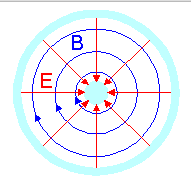
\includegraphics[scale=0.8]{22_1}$  \quad \quad \quad    $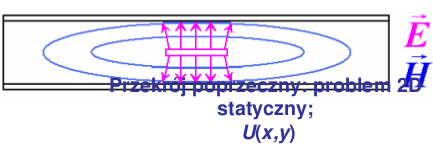
\includegraphics[scale=0.8]{22_2}$\\
	\caption{Linia współosiowa}       \qquad \qquad \qquad  \caption{Linia symetryczna paskowa}\\
%\end{floatingfigure}

%\begin{floatingfigure}
	$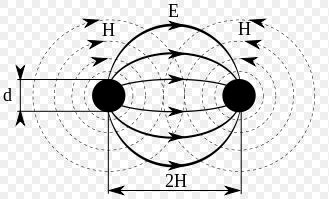
\includegraphics[scale=0.8]{22_3}$ \\
	\caption{Linia dwuprzewodowa symetryczna}\\
%\end{floatingfigure}\\
\textbf{Cechy charakterystyczne:}\\
poziom impedancji charakterystycznej: $Z_{c}=\cfrac{Z}{2\pi}\ln{\cfrac{a}{b}}$, w praktyce stosujemy linie współosiowe o impedancji od 30 $\Omega$ do 100 $\Omega$, najczęściej 50 $\Omega$.\\ 
\textbf{Cechy linii współosiowej:}
\begin{itemize}
\item dobre ekranowanie od pól zewnętrznych (na zewnątrz linii pole elektromagnetyczne jest równe zeru)
\item ograniczony zakres impedancji charakterystycznych
\item trudno robić rozgałęzienia oraz odcinki linii sprzężonych
\item trudności z dołączeniem elementów skupionych
\end{itemize}
Typowe zakresy częstotliwości: kilkadziesiąt $MHz$ do kilku $GHz$. Czasami stosowana do niskich częstotliwości. Wynika to z faktu, że pola przesyłanej fali, dla tej linii, są dobrze odizolowane od pól zewnętrznych, a więc fala ta nie jest zakłócana z zewnątrz ani też nie zakłóca innych fal rozchodzących się w pobliżu.\\
\textbf{Cechy symetrycznej linii paskowej:}\\
Znaczne ułatwienie w budowaniu rozgałęzień i linii sprzężonych w stosunku do linii współosiowej. Stosowana między innymi do budowy filtrów i sprzęgaczy falowych.\\
Przy odpowiednio szerokich płytkach ekranujących (górnej i dolnej o jednakowym potencjale) możemy uznać, że pole, podobnie jak w linii współosiowe jest zamknięte wewnątrz linii, a więc dobrze odseparowane od otoczenia.\\
\textbf{Cechy symetrycznej linii dwuprzewodowej:}\\
Linia ta znajduje zastosowanie w energetyce. Stosuje się ją w zakresie wielkich częstotliwości. Wadą tej linii jest rozproszenie pola na zewnątrz, a więc możliwość sprzężeń przesyłanego sygnału z innymi sygnałami elektronicznymi.

Zalety:
\begin{itemize}
\item prostota budowy
\item możliwość realizowania linii o dużej impredancji charakterystycznej (rzędu kilkuset $\Omega$)
\end{itemize}
Taka linia jest stosowania do połączeń odbiorników telewizyjnych z antenami.\\

\textbf{Obliczanie pojemności przewodu:}\\
$$C_{1}=\cfrac{2\pi\epsilon_{0}}{\ln{\cfrac{a}{b}}}$$
$$Z_{c}=\cfrac{Z_{0}}{2\pi}\ln{\cfrac{a}{b}} \ \ \ \ \ \ \ln{\cfrac{a}{b}}=\cfrac{Z_{c}}{Z_{0}}2\pi$$
$$C_{1}=\cfrac{Z_{0}\epsilon_{0}}{Z_{c}}=\cfrac{1}{15} \cfrac{nF}{m}$$


\end{solution}

\section*{Zadanie 23.}
\begin{task}
Przedyskutować fizyczne efekty związane z prawem Faraday`a.
\end{task}

\begin{solution}
Pod wpływem zmian strumienia magnetycznego powstaje w ramce przewodzącej siła elektromotoryczna równa co do wartości szybkości zmian strumienia magnetycznego. Zwrot siły elektromotorycznej jest taki, że spowodowany przez nią prąd wywołuje pole magnetyczne przeciwstawiające się zmianom pola zewnętrzengo.
Po uwzględnieniu znaku, siła elektromotoryczna wyraża się wzorem:
$$ V = \cfrac{-\partial\varphi}{\partial t}$$
$$ V = \oint_{l}\vec{E}d\vec{l} $$
$$ \varphi = \iint_{S}\vec{B}\vec{n}ds$$
\begin{center}
$\oint_{l}\vec{E}d\vec{l}=-\iint_{S}\cfrac{\partial\vec{B}}{\partial t}\vec{n}ds $ - I równanie Maxwella\\

    $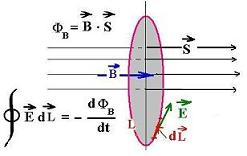
\includegraphics[scale=1]{23}$\\
    \end{center}
\end{solution}

\section*{Zadanie 25.}
\begin{task}
Falowód prostokątny o bokach $a = 5 cm$ i $b = 2.5 cm$ jest wypełniony bezstratnym dielektrykiem o poszukiwanej względen przenikalności elektrycznej $\varepsilon_w$. Stwierdzono, że dla częstotliwości dwa razy wiekszej od częstotliwości granicznej długość fali w falowodzie jest równa długości fali w próżni. Obliczyć $\varepsilon_w$. Który rodzaj fali e.m. rozchodzi się w falowodzie (uazasadnić) ?
\end{task}

\begin{solution}

$f = 2 \cdot f_g$ $\qquad$
$\lambda_{w \ falowodzie} = \lambda_{w \ prozni}$ \\
$\lambda_{w \ falowodzie} = \frac{2 \pi}{\beta_z} = \frac{\frac{2 \pi}{\beta}}{\sqrt{1-(\frac{\beta_g}{\beta})^2}} =  \frac{\lambda}{\sqrt{1-(\frac{\lambda}{\lambda_g})^2}} = \frac{\lambda}{\sqrt{1-(\frac{\omega_g}{\omega})^2}} = \frac{\lambda}{\sqrt{1-(\frac{f_g}{f})^2}}$ \\
$\lambda_{w \ falowodzie} =  \frac{\lambda}{\sqrt{1-(\frac{f_g}{f})^2}} \stackrel{\substack{f = 2 \cdot f_g}}{=} \frac{\lambda}{\sqrt{1-(\frac{\not f_g}{2 \not f_g})^2}} = \frac{\lambda}{\sqrt{1-(\frac{1}{2})^2}} = \frac{\lambda}{\sqrt{1-\frac{1}{4}}} = \frac{\lambda}{\sqrt{\frac{3}{4}}}$ \\ \\
$\lambda_{w \ prozni} = \frac{c}{f}$ \\ \\
$\lambda = \frac{c}{\sqrt{\varepsilon_w} \cdot f}$ \\ \\
$\lambda_{w \ falowodzie} = \lambda_{w \ prozni} \qquad \Rightarrow \qquad  \frac{\frac{\not c}{\sqrt{\varepsilon_w} \cdot \not f}}{\sqrt{\frac{3}{4}}} = \frac{\not c}{\not f} \qquad \Rightarrow \qquad \frac{\frac{1}{\sqrt{\varepsilon_w} }}{\sqrt{\frac{3}{4}}} = 1 \qquad \Rightarrow \qquad \frac{\frac{1}{\varepsilon_w }}{\frac{3}{4}} = 1 = \qquad \Rightarrow \qquad \varepsilon_w  = {\frac{4}{3}} $ \\ \\

\textit {Nie da się okreslić rodzaju fali e.m. jaka rozchodzi sie w falowodzie, jest za mało danych. Wymiary falowodu były podane "dla zmyłki"}  dr J.Piotrowski 2014


\end{solution}
\section*{Zadanie 26.}
\begin{task}
W niemagnetycznym ($\mu=\mu_{0}$) ośrodku o impedancji $Z=|Z|e^{j\cfrac{\pi}{6}}$ rozchodzi się
fala o wektorze pola magnetycznego $\vec{H}=(\vec{i_{x}} + j\vec{i_{y}})H_{0}e^{-\alpha x}e^{j(\omega t - \beta z)}$, gdzie $H_{0}$ - rzeczywiste.
\begin{enumerate}[a)]
\item Obliczyć wektor rzeczywisty $\vec{E}$ i narysować krzywą zakreślaną przez koniec
            tego wektora w płaszczyźnie $0xy \ (z=0)$ 
\item Zakładając, ze znamy $Z, \ \alpha, \ \beta $ oraz $H_{0}$ podać wzór na zależność 
            od czasu wartości powierzchniowej gęstości mocy tej fali w płaszczyźnie $z=2m$.\\ \\
\textbf{Uwaga: Można wybrać (po uprzednim zaznaczeniu) łatwiejszą wersję zadania z założeniem
ośrodka bezstratnego (Z rzeczywiste, $\alpha=0$) z oceną maksymalną 10 p.} \\
\end{enumerate}
\end{task}

\begin{solution}
$$ \vec{H} = (\vec{i_{x}} + j\vec{i_{y}})H_{0}e^{-\alpha x}e^{j(\omega t - \beta z)} = \vec{i_{x}}H_{0}e^{-\alpha x}e^{j(\omega t - \beta z)} + \vec{i_{y}}H_{0}e^{-\alpha x }e^{j(\omega t - \beta z + \cfrac{\pi}{2})} $$
$$\vec{E}=Z(\vec{H}\times\vec{k})=ZH_{0}e^{-\alpha z} \begin{vmatrix}
					\vec{i_{x}}&\vec{i_{y}}&\vec{i_{z}}\\
					e^{j(\omega t-\beta z)}&e^{j(\omega t-\beta z+\cfrac{\pi}{2})}&0\\
					0&0&1\end{vmatrix}
					=ZH_{0}e^{-\alpha z}[\vec{i_{x}}e^{j(\omega t - \beta z + \cfrac{\pi}{2})} - 
							\vec{i_{y}}e^{j(\omega t - \beta z)}]=$$ $$
					|Z|e^{j\cfrac{\pi}{6}}H_{0}e^{-\alpha z}[\vec{i_{x}}e^{j(\omega t - \beta z + \cfrac{\pi}{2})} - 
							\vec{i_{y}}e^{j(\omega t - \beta z)}]
					=|Z|H_{0}e^{-\alpha z}\big{[}\vec{i_{x}}e^{j(\omega t - \beta z + \cfrac{\pi}{2} + 
					\cfrac{\pi}{6})} - \vec{i_{y}}e^{j(\omega t - \beta z + \cfrac{\pi}{6})}\big{]}$$
Postać rzeczywista:
$$\vec{H_{r}}=H_{0}e^{- \alpha z}(\vec{i_{x}}\cos(\omega t - \beta z) - \vec{i_{y}}
				\sin(\omega t - \beta z)) $$
$$\vec{E_{r}}=|Z|H_{0}e^{- \alpha z}\big{(}-\vec{i_{x}}\cos(\omega t - \beta z + 
					\cfrac{\pi}{6}) - \vec{i_{y}}\sin(\omega t - \beta z + \cfrac{\pi}{6})\big{)} $$\\
Wektor Poyntinga:

$$\vec{S}=\vec{E}\times\vec{H}=|Z|H_{0}^{2}e^{-2\alpha z}\begin{vmatrix}
					\vec{i_{x}}&\vec{i_{y}}&\vec{i_{z}}\\
					-\sin{(\omega t-\beta z+\cfrac{\pi}{6})}&-\cos{(\omega t-\beta z+\cfrac{\pi}{6})}&0\\
					\cos(\omega t - \beta z)&-\sin(\omega t - \beta z)&0\end{vmatrix}=$$\\
					$$=H_{0}^{2}|Z|e^{2\alpha z}\vec{i_{z}}(\sin(\omega t - \beta z + \cfrac{\pi}{6})\sin(\omega t - \beta z) + \cos(\omega t - \beta z)\cos(\omega t - \beta z + \cfrac{\pi}{6}) )$$

\begin{center}
$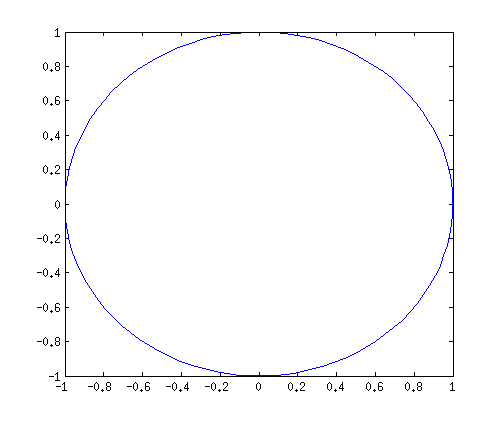
\includegraphics[scale=0.7]{26_1}$\\
\end{center}

$$\vec{S}(z=2m)=H_{0}^{2}|Z|e^{4\alpha}\vec{i_{z}}(\sin(\omega t - 2\beta + \cfrac{\pi}{6})\sin(\omega t - 2\beta) + \cos(\omega t - 2\beta)\cos(\omega t - 2\beta + \cfrac{\pi}{6}) )$$

\end{solution}

\section*{Zadanie 27.}
\begin{task}
Obliczyć długość fali elektromagnetycznej o częstotliwości f=30 MHz
\begin{enumerate}[a)]
\item w dielektryku o $\epsilon_{w}=9$, $\mu_{w}=1$, $\sigma=0$
\item w przewodniku o $\epsilon_{w}=1$, $\mu_{w}=1$, $\sigma=10^{7} \ \cfrac{S}{m}$
\item w plaźmie o częstotliwości własnej plazmy $f_{p}=20\ MHz$
\item w plaźmie o częstotliwości drgań własnych $f_{p}=50\ MHz$
\end{enumerate}
Uwaga: $\mu_{0}=4\pi10^{-7} \cfrac{H}{m}$\\
Krótko omówić fizyczne interpretacje otrzymanych wyników.\\
\end{task}

\begin{solution}
\begin{enumerate}[a)]
\item $\lambda=\cfrac{1}{f\sqrt{\mu\epsilon}}=\cfrac{c}{f\sqrt{\mu_{w}\epsilon_{w}}}=\cfrac{10}{3} \ m$
\item $v=\cfrac{\omega}{\beta}$ $\lambda=
            \cfrac{2\pi}{\beta}=\cfrac{2\pi}{\sqrt{\cfrac{\omega\mu\sigma}{2}}}\\ \lambda=\cfrac{1}{\sqrt{30}}*10^{-3}\ m$
\item $\epsilon_{p}=\epsilon_{0}[1-(\cfrac{\omega_p}{\omega})^{2}]=\epsilon_{0}[1-(\cfrac{f_{p}}{f})^{2}]$\\
                $\lambda_{p}=\cfrac{\lambda_{0}}{\sqrt{\epsilon_{p}}}=\cfrac{c}{f\sqrt{\epsilon_{0}[1-(\cfrac{f_{p}}{f})^{2}]}}$
\item Fala się nie rozchodzi, bo $\omega<\omega_{p}$

\end{enumerate}
\end{solution}



\section*{Zadanie 29.}
\begin{task}
Fala płaska biegnąca w kierunku \textsl{Ox} i spolaryzowana liniowo tak, że pole elektryczne jest równoległe do
osi \textsl{Oy} i ma amplitudę 1V/m, pada prostopadle na płytę idealnie przewodzącą, umieszczoną w 
płaszczyźnie x=0. Zapisać rzeczywistą postać wyrażeń na pole \textsl{E} i \textsl{H} dla fali padającej,
odbitej i przechodzącej. Obliczyć gęstość powierzchniową prądu płynącego po płycie. Narysować obwiednie dla
pola \textsl{E} i \textsl{H}. Wyjaśnić, co zmieni się, gdy płyta będzie miala przewodność właściwą $\sigma$
dużą, ale ograniczoną. Narysować obwiednie pól \textsl{E} i \textsl{H} w płycie dla dwóch różnych wartości 
$\sigma_{1}$ oraz $\sigma_{2}=2\sigma_{1}$.\\ \\
\end{task}

\begin{solution}
Postać rzeczywista \textsl{E} i \textsl{H}:
\begin{itemize}
\item $\vec{E^{+}_{1}}=\vec{i_{y}}E_{0}cos(wt-\beta x)$\\
       $\vec{E^{-}_{1}}=-\vec{i_{y}}E_{0}cos(wt+\beta x)$\\
       $\vec{E_{2}}=0$
\item $\vec{H^{+}_{1}}=\vec{i_{z}}H_{0}cos(wt-\beta x)$\\
       $\vec{H^{-}_{1}}=\vec{i_{z}}H_{0}cos(wt+\beta x)$\\
       $\vec{H_{2}}=0$\\ \\
\end{itemize}

Obwiednia pól dla idealnego przewodnika:\\
\begin{center}
$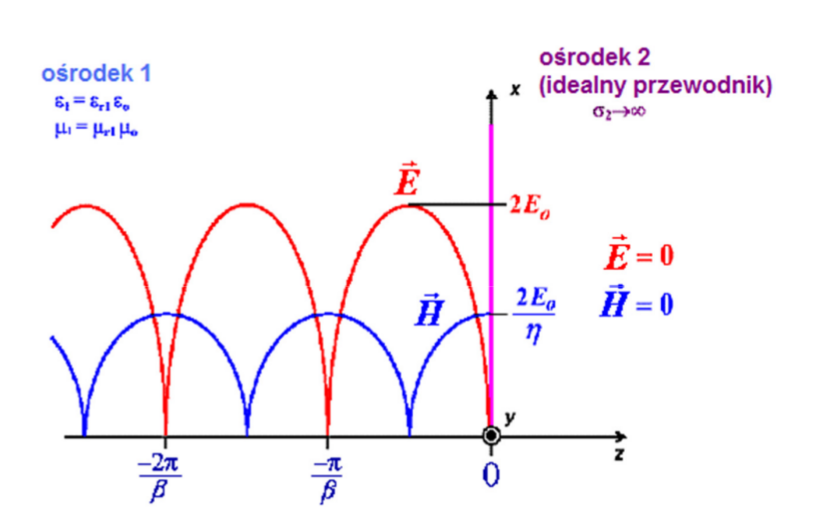
\includegraphics[scale=0.7]{29_1}$\\
\end{center}

Obliczamy gęstość prądu:
$$\vec{n}\times(\vec{H_{2}} - \vec{H_{1}})=\vec{J}$$
$$\vec{H_{2}} = 0$$
$$H_{0} = J$$
Dla wartości $\sigma_{1}$ odwiednia pól \textsl{E} i \textsl{H} maleje wolniej niż dla wartości
$\sigma_{2}=2\sigma_{1}$.\\
Rozkład amplitud dla przykładowej wartości $\sigma$:
\begin{center}
$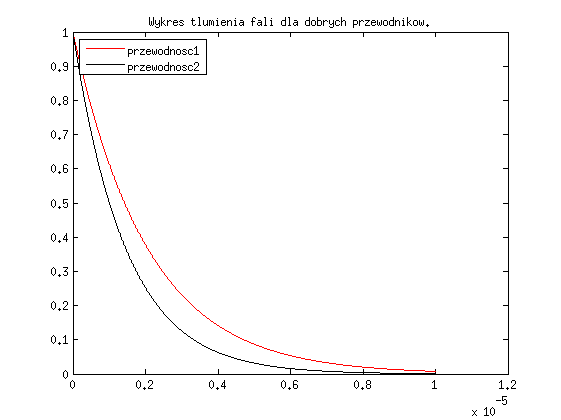
\includegraphics[scale=0.9]{29_2}$\\
\end{center}

\end{solution}

\section*{Zadanie 33.}
\begin{task}
Narysować (w przekroju poprzecznym oraz pionowym i poziomym przekroju wzdłużnym) rozkłady pól 
$\textsl{E}$ i $\textsl{H}$ oraz prądów przewodzenia i przesunięcia dla fali bieżącej rodzaju $E_{01}$
w falowodzie kołowym. Jaki rodzaj w falowodzie prostokątnym  jest fizycznym odpowiednikiem tego rodzaju?\\
\end{task}

\begin{solution}

\begin{center}
$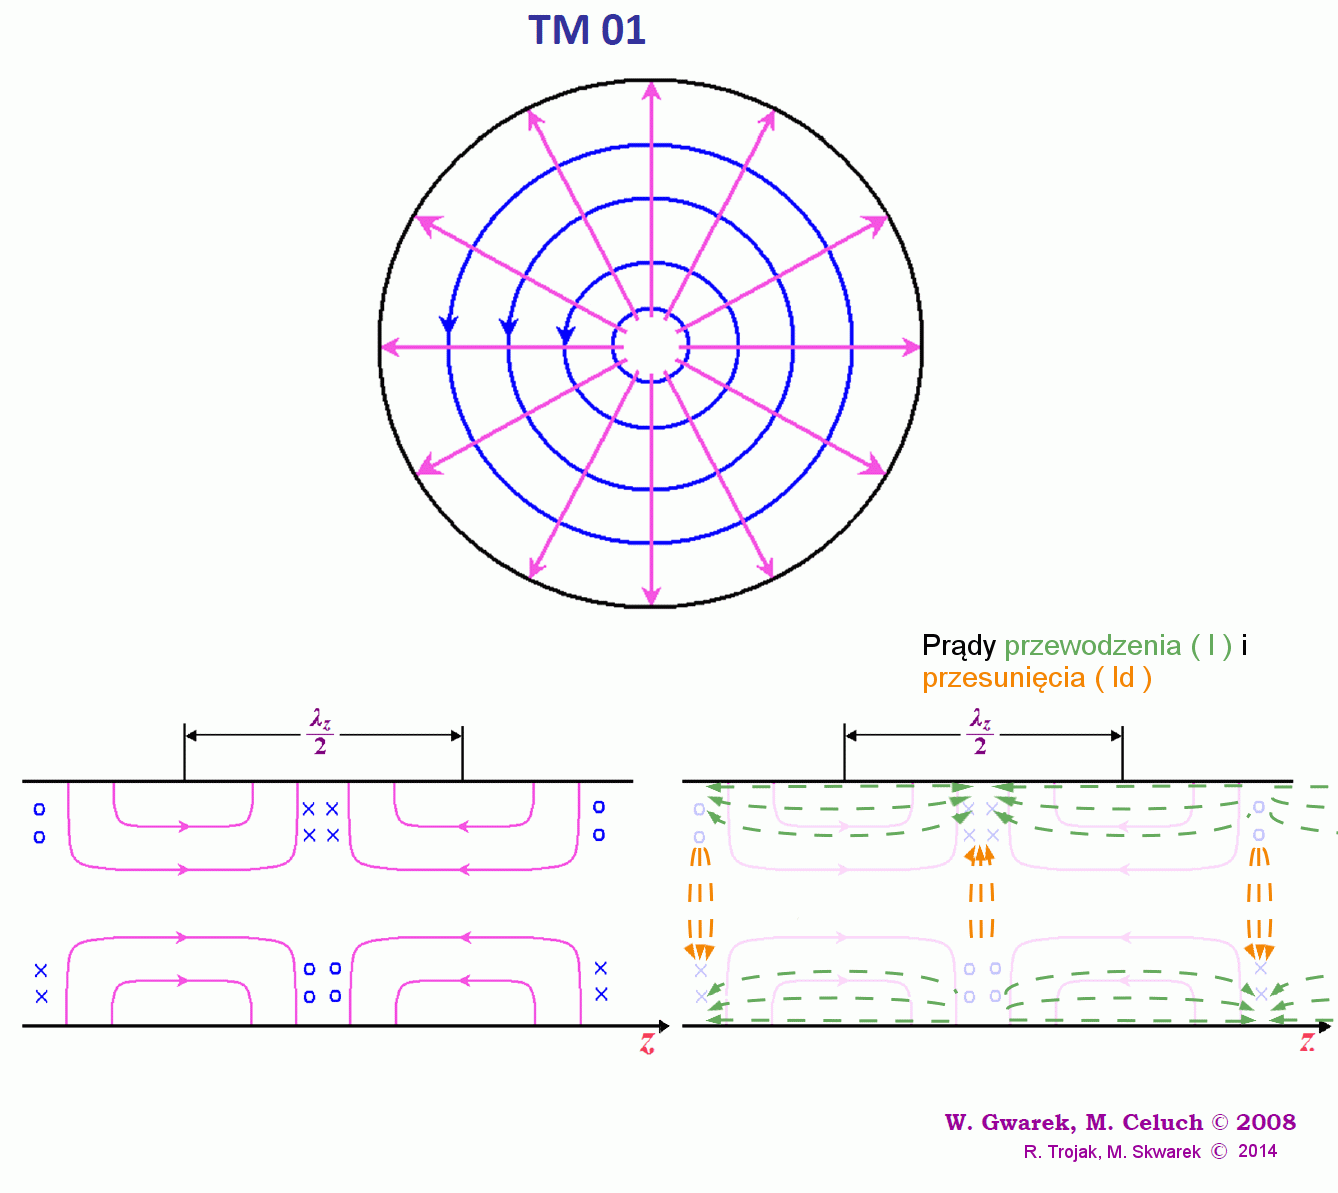
\includegraphics[scale=0.4]{33_1}$\\
\end{center}
Odpowiednikiem tego rodzaju w falowodzie prostokątnym jest rodzaj $E_{11}$\\
\end{solution}

\section*{Zadanie 35.}
\begin{task}
	Wyjaśnić do czego wykorzystuje się rozwiązanie równania Laplace`a w teorii linii TEM. Naszkicować pola
	\textsl{E} i \textsl{H} w przekroju najczęsciej stosowanej linii z klasy "quasi-TEM". Wyjaśnić jakie cechy
	i parametry odróżniają ją od tych linii, które dokładnie spelniają założenia klasy TEM.\\
\end{task}

\begin{solution}
	Prowadzona fala TEM - zmienność poprzeczna
	\begin{itemize}
	\item pola są potencjalne (bezwirowe) w płaszczyźnie XY
	\item mogą być opisane jako:$\\\vec{E_{\perp}} = -\nabla_{\perp}U$\ (*)\\
		$\nabla_{\perp}\vec{D}=0$\     $\nabla_{\perp}\vec{E_{\perp}}=0$\\
		co\ prowadzi\ do\ równania\ Laplace`a:\\
		$\nabla_{\perp}^2U=0$    (*1)
	\end{itemize}
	Funkcja otrzymana z równania (*1) pozwala na określenie ${\vec{E_{\perp}}}$ z równania (*)\\
	Z własności rozwiązań równania Laplace`a:
	\begin{itemize}
	\item fale TEM nie mogą się rozchodzić w liniach jednoprzewodowych (z zasady supremum)
	\item rozwiązania z określonymi warunkami brzegowymi są jednoznaczne
	\item zasada superpozycji w liniach wieloprzewodowych\\			
	\end{itemize}
	Metody rozwiązywania równań Laplace`a:
	\begin{itemize}
	\item bezpośrednie całkowanie
	\item rozdzielanie zmiennych
	\item odwzorowanie konforemne
	\item metoda Monte-Carlo	
	\end{itemize}

	Niesymetryczna linia paskowa (linie mikropaskowe (quasi-TEM)\\
	\textbf{przekrój poprzeczny:}\\
	\begin{center}
    $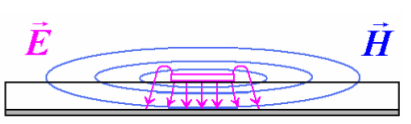
\includegraphics[scale=0.7]{35_1}$\\
    \end{center}
	\textbf{przekrój wzdłużny:}\\
	\begin{center}
    $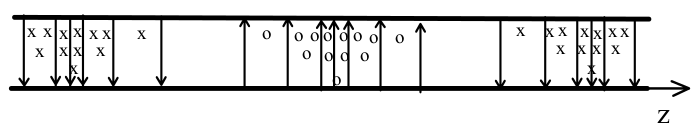
\includegraphics[scale=0.7]{35_2}$\\
    \end{center}
	Cechy niesymetrycznej linii paskowej:
	\begin{itemize}
	\item zależność dlugości fali od szerokości linii
	\item zależność parametrów od częstotliwości (dyspersja)
	\item gorsze odseparowanie od pól zewnętrznych oraz promieniowanie	
	\end{itemize}
\end{solution}
\section*{Zadanie 37}
\begin{task}
Jaki jest zakres stosowalności równań Maxwella. Podać przykłady praktycznych problemów elektroniki które mogą oraz tych które nie mogą być rozwiązane za ich pomocą. Czy wszystkie równania Maxwella mają równie szerokie zastosowania (to znaczy w jakich okolicznościach niektóre z równań są zależne od innych) \\
\end{task}

\begin{solution}
Równania Maxwella - cztery podstawowe równania elektrodynamiki klasycznej zebrane i rozwinięte przez Jamesa Clerka Maxwella. Opisują one właściwości pola elektrycznego i magnetycznego oraz zależności między tymi polami. Z równań Maxwella można wyprowadzić między innymi równania falowe fali elektromagnetycznej oraz wyznaczyć prędkość takiej fali propagującej (rozchodzącej się) w próżni (prędkość światła).


Równania Maxwella w postaci ogólnej 
$$ \nabla \times \vec{E} = -  \frac{ \delta  \vec{B} }{\delta t}  $$
 $$\nabla \times \vec{H} =  \vec{J} + \frac{ \delta  \vec{D} }{\delta t} $$
$$\nabla  \cdot \vec{D} =  \rho $$
$$\nabla  \cdot \vec{E} =  0  $$

Równania Maxwella w postaci całkowej \\
 $$\oint\limits_{l}\vec{E}dl = - \iint\limits_{S}\frac{\delta \vec{B}}{\delta t}$$
 $$\oint\limits_{l}\vec{H}dl =  \iint\limits_{S}( \vec{J} + \frac{\delta \vec{B}}{\delta t} )  $$
$$\oiint\limits_{S} \vec{D} \vec{n} ds = \iiint\limits_{V} \rho dv $$
$$\oiint\limits_{S} \vec{B} \vec{n} ds = 0 $$

Równania Maxwella w postaci zespolonej \\
$$\nabla \times \vec{E} = -j \omega \vec{B} $$
$$\nabla \times \vec{H} = \vec{J} + j\omega\vec{D} $$
$$\nabla \cdot \vec{D} = \rho $$
$$\nabla \cdot \vec{B} = 0 $$


Równania Maxwella tworzą podstawę elektrodynamiki klasycznej oraz podstawę do wyprowadzenia prawa Biota-Savarta. Całkując po czasie I r.M. i biorąc dywergencję IV r.M. otrzymujemy równanie opisujące zasadę zachowania ładunku
$$\nabla \cdot J = -  \frac{\delta \rho}{\delta t} $$

Całkująć II r.M. po powierzchni s której brzegiem L jest obwód elektryczny, dostrzegamy że gdy strumień pola magnetycznego przez s nie zmienia się to II r.M. przyjmuje postac 

$$\int\limits_L \vec{E} dL = 0 $$

i staje się napięciowym prawem Kirhoffa

$$ \int\limits_{a}^{b} \vec{E} dL + \int\limits_{b}^{c}\vec{E} dL + \int\limits_{c}^{d} \vec{E} dL + \int\limits_{d}^{a} \vec{E} dL = 0\\  U_{ab} + U_{bc} + U_{cd} + U_{da} = 0\\ \sum_{i=a}^{d} U_{i}=0  $$

Szczególnie istotne jest II r.M. które jest rozwinięciem Prawa Amprere'a - prawa wiążącego indukcję magnetyczną wokół przewodnika z prądem z natężeniem prądu elektrycznego przepływającego w tym przewodniku. Mówi ono że przepływający w przewodniku prąd wytwarza wokół niego pole magnetyczne. 

$$\nabla \times \vec{H} =  \vec{J} + \frac{ \delta  \vec{D} }{\delta t} $$

Maxwell rozwinął to prawo do postaci polowej, dodając do wyrażenie na prąd przesunięcia

$$J_{D} = \frac{\delta \vec{D}}{\delta t} $$

w wyniku obserwacji że pole magnetyczne tworzy nie tylko przepływający prąd, ale również zmienne pole elektryczne wokół przewodnka (prad przesunięcia).

Dużą rolę ma również I.r.M. wynikające z prawa Faraday'a mówiące o przeciwdziałaniu polu przez je samo, tj. zmienne pole magnetyczne wokół przewodnika indukuje w nim ruch ładunków wytwarzający prąd elektryczny co do wartości równy szybkości zmiany pola magnetycznego o kierunku takim, że indukowane przez niego pole magnetyczne przeciwdziała polu które ruch ładunków wytworzyło.

Jak łatwo zauważyć analizując wzory, wzajemnie zalezne od siebie są I i II oraz III i IV r.M. 
\\

\end{solution}
\section*{Zadanie 38.}
\begin{task}
Co to jest efekt naskórkowy i jak zalezy od częstotliwości. Przedyskutować jakiego rzedu grubości pasków metalowych powinny być stosowane w obwodach drukowanych na zakres ok. 3GHz (takich jak np. szybkie układy cyfrowe)?\\
\end{task}



\begin{solution}
Efekt naskórkowy występuje w sytuacji kiedy pole elektromagnetyczne napotyka przewodnik. Na powierzchni przewodnika wytwarza się prąd. W przypadku napotkania przewodnika idealnego (o nieskończonej konduktywności) prąd wytwarza się na nieskończenie cienkiej wartwie na powierzchni przewodnika. Natomiast w realnych przewodnikach mamy do czynienia z głębokością wnikania, wielkością charakteryzującą efekt naskórkowy, zależną od częstotliwości fali i konduktywności przewodnika.
Głębokość wnikania jest tym większa im mniejsza jest częstotliwość fali elektromagnetycznej, co wynika bezpośredniu ze wzoru na tą wielkość.\\
\\
 $\delta = \frac{1}{ \alpha } \\$
 $\alpha  =  \sqrt{\frac{ \omega    \mu _{0}  \sigma  }{2}} = \sqrt{\frac{ \not{2} \pi f    \mu _{0}  \sigma  }{\not{2}}} = \sqrt {\pi f    \mu _{0}  \sigma}\\$
\\
Najczęśćiej by uniknąć strat przy przewodzeniu prądu, stosuje się przewodniki np. mosiężne, pokryte odpowiednio cienką, ze względu na koszty, warstwą (równą głębokości wnikania) materiału o dużej konduktywności (np. srebro, miedź, złoto).
Przyjmując że przewodnik pokryliśmy srebrem $\sigma_{Ag} = 6 \cdot 10^7 [\frac{S}{m}]$ , dla fali o częstotliwości 3GHz warstwa srebra musi mieć grubość równą: \\
\\
 $\begin{cases} \pi \cong 3.14\\f =3\cdot 10^9 Hz \\\mu _{0} = 4 \cdot \pi \cdot 10^{-7}\\ \sigma_{Ag} = 6 \cdot 10^7 [\frac{S}{m}] \end{cases} \\ \\$
 $\delta_{Ag} = \frac{1}{ \alpha } = \frac{1}{\sqrt {\pi f    \mu _{0}  \sigma}} = \frac{1}{\sqrt {\pi \cdot 3\cdot 10^9 \cdot 4 \cdot \pi \cdot 10^{-7} 6 \cdot 10^7}} = 1.186 \cdot 10^{-6} m \\$

\end{solution}
\section*{Zadanie 39.}
\begin{task}
Jakie są właściwości elektryczne zimnej plazmy? Gdzie występuje ona w przyrodzie? Jaki ma wpływ na propagację fal radiowcyh w atmosferze? ( z wyróżnieniem własności fal długich, krótkich, UKF i mikrofal) ?\\
\end{task}


\begin{solution}
Plazma – zjonizowana materia o stanie skupienia przypominającym gaz, w którym znaczna część cząstek jest naładowana elektrycznie. Mimo że plazma zawiera swobodne cząstki naładowane, to w skali makroskopowej jest elektrycznie obojętna.
Plazma zimna powstaje przy odpowiednio niskich temperaturach i gęstościach, w warunkach ziemskich (na przykład podczas wyładowań atmosferycznych - znajduje się ona zatem w jonosferze) i w zbudowanych przez człowieka urządzeniach (na przykład plazmotronach). W jej skład, prócz składników tworzących plazmę gorącą, wchodzić mogą również atomy i ich jony, a także cząsteczki (zarówno obojętne, jak i zjonizowane).\\
Warunki w plazmie.\\
\begin{textbf} {1.}\end{textbf} Fale o $\omega < \omega_{p}$ są tłumione w plazmie. W przypadku padania fali o takiej omedze z próżni na warstwę jonosfery ulegnie ona całkowitemu odbiciu.\\
\begin{textbf} {2.}\end{textbf} Fale i $\omega > \omega_{p}$ rozchodzą się w plazmie. W przypadku padania fali ukośnie z próżni na jonosferę fala załamania odchyla sie od normalnej(gdyż przechodzi do ośrodka rzadszego)\\
\begin{textbf} {3.}\end{textbf} Fale o $\omega >> \omega_{p}$ rozchodzą się w plazmie tak jak w próżni, ponieważ $\varepsilon_{p} \longrightarrow \varepsilon_{0}$. Tylko takie fale (w prakrtyce - mikrofale) swobodnie przechodzą przez jonosferę i mogą być użyte w komunikacji satelitarnej.\\
PRZYPOMNIENIE: Im mniejsza długość fali, tym większa jej częstotliwość/energia/pulsacja drgań własnych\\
Fale długie (od 100m do 2000m) rozchodzą się nisko po powierzchni ziemi, zimna plazma zawarta w jonosferze nie wpływa na ich propagację.\\
Fale krótkie (od 10m do 100m) mają własność odbijania się od górnych warstw atmosfery (m.in. jonosfery). Plazma zamawrta w jonosferze sprawia że zgodnie z warunkiem \begin{textbf} {(1.)}\end{textbf} fale te odbijają się od jonosfery co umożliwia im osiągnąć globalny zasięg.\\
UKF - "Ultra Krótkie Fale" (od 10cm do 1m) - ich pulsacja jest większa od pulsacji własnej plazmy, więc zgodnie z warunkiem \begin{textbf} {(2.)}\end{textbf}  fale w jonosferze "przechodzą dalej" (z załamaniem ) i nie następuje ich odbicie z powrotem do odbiorników/nadajników. Powoduje to że fale te mają jedynie zasięg jaki umozliwia rozsyłanie ich liniowo, stosowane są w radiostacjach.\\
Mikrofale (do 30cm) - dale te mają bardzo dużą częstotliwość przez co ich pulsacja drgań własnych jest duzo wieksza od tej wielkośći w plazmie. Zgodnie z warunkiem \begin{textbf} {(3.)}\end{textbf} fale przechodzą przez zimną plazmę zawartą w jonosferze jak przez próżnię (nie załamują się) co umożliwia użycie tych fal w astrologii (np. radioteleskopy).

\end{solution}
\section*{Zadanie 40.}
\begin{task}
Fala płaska rozchodząca się w kierunku $+Ox$ pada prostopadle na granice w układzie trzech ośrodków:\\
I $\hspace{1cm}$ $\varepsilon_{1}=\epsilon_{0} \hspace{1.2cm} \mu_{1}=\mu_{0} \hspace{1cm} \sigma=0 \hspace{4cm}$ dla $x<-d$\\
II $\hspace{0.86cm}$ $\epsilon_{2}=3\epsilon_{0} \hspace{0.95cm} \mu_{2}=? \hspace{1.35cm} \sigma=0 \hspace{4cm}$ dla $-d\le x<0$\\
III $\hspace{0.72cm}$ $\epsilon_{3}=? \hspace{1.4cm} \mu_{3}=5\mu_{0} \hspace{0.83cm} \sigma=0 \hspace{4cm}$ dla $0\le x$\\
gdzie d=7.5cm.\\
Wiedząc, że współczynnik fali stojącej w ośrodku I wynosi jeden w zakresie częstotliwości od 8 GHz do 12 GHz wyznaczyć wartości $\mu_{2}$ i $\epsilon_{3}$. Dla częstotliwości 10GHz obliczyć długość fali w ośrodku II i narysować obwiednię natężenia pola elektrycznego znormalizowaną do amplitudy $E_{30}$ natężenie pola elektrycznego fali w ośrodku III.\\
\end{task}

\begin{solution}

\textbf{Obliczanie parametrów ośrodka:}
$$WFS_{1}=1 \ \ \ \implies \ \ \ \Gamma_{1,2}=0$$
$$\Gamma_{1,2}=0 \ \ \ \implies \ \ \ Z_{in}=Z_{1} \ \ \ \implies \ \ \ Z_{2}\cfrac{Z_{3}+jZ_{2}\tg{\beta_{2}d}}{Z_{2}+jZ_{3}\tg{\beta_{2}d}}=Z_{1}$$
$\left\{ \begin{array}{l} Z_{1}=\sqrt{\cfrac{\mu_{1}}{\epsilon_{1}}}Z_{0}\\Z_{2}=\sqrt{\cfrac{\mu_{2}}{\epsilon_{2}}}Z_{0}\\Z_{3}=\sqrt{\cfrac{\mu_{3}}{\epsilon_{3}}}Z_{0}  \end{array} \leftarrow \ \mu_{x} \ \epsilon_{x}$ traktujemy jako liczby, współczynniki przy $\epsilon_{0} \ \mu_{0}$ \\ Podstawiamy i wymnażamy obie strony przez mianownik:\\
$$\sqrt{\cfrac{\mu_{2}}{\epsilon_{2}}}Z_{0}\big{(}\sqrt{\cfrac{\mu_{3}}{\epsilon_{3}}}Z_{0}+j\sqrt{\cfrac{\mu_{2}}{\epsilon_{2}}}Z_{0}\tg{\beta_{2}d}\big{)}=\sqrt{\cfrac{\mu_{1}}{\epsilon_{1}}}Z_{0}\big{(}\sqrt{\cfrac{\mu_{2}}{\epsilon_{2}}}Z_{0}+j\sqrt{\cfrac{\mu_{3}}{\epsilon_{3}}}Z_{0}\tg{\beta_{2}d}\big{)}$$
$$\sqrt{\cfrac{\mu_{2}\mu_{3}}{\epsilon_{2}\epsilon_{3}}} +j\cfrac{\mu_{2}}{\epsilon_{2}}\tg{\beta_{2}d} = \sqrt{\cfrac{\mu_{1}\mu_{2}}{\epsilon_{1}\epsilon_{2}}}+j\sqrt{\cfrac{\mu_{1}\mu_{3}}{\epsilon_{1}\epsilon_{3}}}\tg{\beta_{2}d} $$
Porównujemy liczby zespolone ($ \Re(z_{1})=\Re(z_{2}) $ oraz $ \Im(z_{1})=\Im(z_{2})$) i podstawiamy wartości liczbowe! ($\epsilon_{0}$ oraz $\mu_{0}$ skróciliśmy w $Z_{0}$)\\
$$\left\{ \begin{array}{l} \sqrt{\cfrac{5\mu_{2}}{3\epsilon_{3}}}=\sqrt{\cfrac{\mu_{2}}{3}}\\ \cfrac{\mu_{2}}{3}=\sqrt{\cfrac{5}{\epsilon_{3}}} \end{array}\ \ \ \implies \ \ \  \left\{ \begin{array}{l} \epsilon_{3}=5\\ \mu_{2}=3 \end{array}$$\\
\textbf{Obliczanie długości fali w ośrodku 2:}
$$ \cfrac{\omega}{\beta} = \cfrac{1}{\sqrt{\mu\epsilon}}\ \ \ \implies \ \ \ \beta=\cfrac{\omega}{\cfrac{1}{\sqrt{\mu\epsilon}}}, \ \ \ \ \lambda=\cfrac{2\pi}{\beta} $$
$$ \beta_{2}=\cfrac{3\omega_{2}}{c}=200\pi\ \ \ \ \implies \lambda_{2}=\cfrac{2\pi}{200\pi}=0.01m $$
	\begin{center}
    $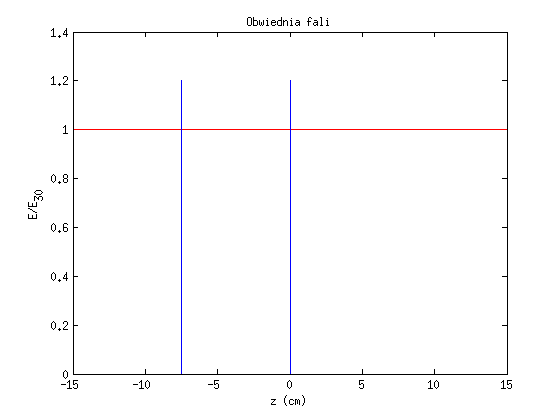
\includegraphics[scale=1]{40}$\\
    \end{center}

\end{solution}
\section*{Zadanie 41.}
\begin{task}

Fala płaska rozchodząca sie w kierunku +0x pada prostopadle na granice w układzie trzech ośrodków:\\
$I \hspace{16} \varepsilon_{1} = \varepsilon_{0} \hspace{30} \mu_{1}=\mu_{0} \hspace{30} \sigma_{1} = 0 $\\
$II \hspace{10} \varepsilon_{2} = 4\varepsilon_{0} \hspace{25} \mu_{2} =\quad ? \hspace{26.5} \sigma_{2} = 0 $\\
$III \ \varepsilon_{3} =\quad ? \hspace{25} \mu_{3}=8\mu_{0} \hspace{25} \sigma_{3} = 0 $\\
gdzie d = 2.5 cm\\
Współczynnik odbicia dla x=0 jest równy 1/3. Wiedząc, że dla pewnej częstotliwości $ f $ grubość ośrodka II stanowi połowę długości fali w tym ośrodku i współczynnik fali stojącej w ośrodku I wynosi jeden wyznaczyć wartości $f, \mu_{2} $ i $ \varepsilon_{3}$. Dla wyznaczonej czestotliwości narysować obwiednię natężenia pola elektrycznego znormalizowaną do amplitudy $E_{30}$ natęzenia pola elektrycznego fali w ośrodku III.\\
\end{task}

\begin{solution}
Współczynnik odbicia dla x=0 jest równy 1/3 (x=0 znajduje się na granicy ośrodków 2 i 3) 
\begin{center}
$\Downarrow $\\
\end{center}
$\Gamma_{2,3} = \frac{Z_{3}-Z_{2}}{Z_{3}+Z{2}} = \frac{1}{3} $\\
$3(Z_{3}-Z_{2}) = Z_{3}+Z_{2}$\\
$3Z_{3}-3Z_{2} = Z_{3}+Z_{2}$\\
$2Z_{3} = 4Z_{2}$\\
$Z_{3} = 2Z_{2}$\\
$\sqrt{\frac{\mu_{3}}{\varepsilon_{3}}} = 2\sqrt{\frac{\mu_{2}}{\varepsilon_{2}}} \quad / ()^{2}$ \\
$\frac{ \mu_{3} }{ \varepsilon_{3} } = 4\frac{\mu_{2}}{\varepsilon_{2}} \qquad \begin{cases} \mu_{3}=8\\\varepsilon_{2}=4\end{cases}$ \\
$ \frac {8}{\varepsilon_{3}} = \not 4 \frac{\mu_{2}}{\not 4} $ \\
$ \mu_{2} = \frac{8}{\varepsilon_{3}}$ \\

dla pewnej częstotliwości f grubość ośrodka II stanowi połowę długości fali w tym ośrodku $\rightarrow$ oznacza to że w ośrodku II mamy do czynienia z tranformatorem półfalowym, czyli takim że $d = \frac{\lambda}{2} \Longleftrightarrow  Z_{1}=Z{3}$\\
z tego wyznaczamy wartość $\varepsilon_{3}$ w nastepujący sposób:\\
$\frac{ \mu_{1} }{ \varepsilon_{1} } = \frac{\mu_{3}}{\varepsilon_{3}}$\\
$1 = \frac{\mu_{3}}{\varepsilon_{3}}$\\
$\varepsilon_{3} = \mu_{3} = 8$\\
$\varepsilon_{3} = 8 \varepsilon_{0} $\\
$\begin{cases} \mu_{2}=1 \quad [\frac{H}{m}]\\\varepsilon_{3}=8 \quad [\frac{F}{m}]\end{cases}$\\
Częstotliwość obliczamy z podstawowego wzoru na częstotliwość fali, tj.
$\lambda = \frac{v}{f} \rightarrow f = \frac{v}{\lambda}$\\
$f = \frac{3 \cdot 10^{8} \frac{m}{s}}{ \sqrt{\mu_{2} \varepsilon_{2}} \cdot 0.05 \ m} = 3 \cdot 10^{9} \ \frac{1}{s} = 3 \cdot 10^{9} \ Hz = 3 \ GHz$\\
\begin{center}
    $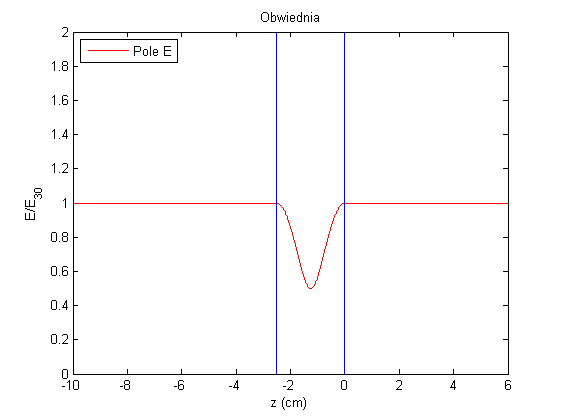
\includegraphics[scale=1]{41}$\\
\end{center}
\end{solution}


\end{document}